\documentclass[tikz,10pt]{standalone}

\usepackage[utf8]{inputenc}
%=======================================================================
%%% Fonts used in this PhD thesis

\usepackage[T1]{fontenc}

\usepackage{csquotes}
\usepackage[english]{babel}

%% serif, as a main font %%
\usepackage{crimson}

%% sans serif, as decoration %%
\usepackage{roboto} %figure caption fonts

% math font
%\usepackage[libertine]{newtxmath} 
%%%%%%%%%%%%%%%%%%%%%%%%%%%%%%%%%%%%%%%%%%%%%%%%%%%%
% MATRIX NOTATION AND MATHS NOTATION
%%%%%%%%%%%%%%%%%%%%%%%%%%%%%%%%%%%%%%%%%%%%%%%%%%%%%
\usepackage{amsmath,amssymb,amsfonts}
\newcommand{\matr}[1]{\mathbf{#1}} % undergraduate algebra version
%\newcommand{\matr}[1]{#1}          % pure math version
%\newcommand{\matr}[1]{\bm{#1}}     % ISO complying version - I need a the bm package for that version 
\newcommand{\euler}{\mathrm{e}}
\newcommand{\inftsml}{\mathrm{d}}
\newcommand{\cmplxnum}{\mathrm{j}}
\newcommand{\setangles}{\mathbb{S}}
\newcommand{\realnumbers}{\mathbb{R}}
%\newcommand{\realnumbers}{\rm I\!R}
\newcommand{\realpart}{\mathrm{Re}}
\newcommand{\complexpart}{\mathrm{Im}}
%\newcommand{\complexnumbers}{\rm I\!I}
\newcommand{\complexnumbers}{\mathbb{C}}

\usepackage{nicefrac}

%small bullet
% https://tex.stackexchange.com/questions/389238/is-there-a-black-dot-symbol-that-i-can-use
\usepackage{scalerel}
\newcommand\sbullet[1][.5]{\mathbin{\ThisStyle{\vcenter{\hbox{
					\scalebox{#1}{$\SavedStyle\bullet$}}}}}
}

\usepackage{mathtools} % \colloneq
%%%%%%%%%%%%%%%%%%%%%%%%%%%%%%%%%%%%%%%%%%%%%%%%%%%%%


% calligraphical font
\usepackage{calligra}

% hiragana/kanji
\usepackage{CJKutf8}



\usepackage{graphicx} % [draft]{graphicx} to remove all images
\graphicspath{ {images/} }
\usepackage{wrapfig}

\usepackage{breakcites}

\usepackage[strict]{changepage} % for CV. As the "section" of bch font is slightly off the balance compared with "main text" of crimson font. the balance is then fixed by placing the bch font in the main text, and the "section" of bch font is adjusted accordingly.

%=======================================================================
%%% thesis geometry

%\usepackage[text={115mm,197.2mm},hmarginratio=1:1,vmarginratio=1:1,marginparwidth=12mm]{geometry} 

%=======================================================================

%\usepackage{lipsum} %generating lorem ipsum
%\usepackage{kantlipsum}


%%%%%%%%%%%%%%%%%%%%%%%%%%%%%%%%%%%%%%%%%%%%%%%%%%%%%
% Units
%%%%%%%%%%%%%%%%%%%%%%%%%%%%%%%%%%%%%%%%%%%%%%%%%%%%%
\usepackage{siunitx}
\DeclareSIUnit \voltampere { VA } %apparent power
\DeclareSIUnit \voltamperereactive { var } %var %https://www.electropedia.org/iev/iev.nsf/display?openform&ievref=131-11-45
\DeclareSIUnit \watthour { Wh } %watt hour
\DeclareSIUnit \perunit { pu } %per unit
\DeclareSIUnit \degree { \ensuremath{^\circ} } %per unit
%%%%%%%%%%%%%%%%%%%%%%%%%%%%%%%%%%%%%%%%%%%%%%%%%%%%%

\usepackage{setspace}
\usepackage{booktabs}

%\usepackage{emptypage} %remove header, footer along with the page number in an empty page
%\newcommand\mybar{\kern1pt\rule[-\dp\strutbox]{1pt}{\baselineskip}\kern1pt} %vertical bar
%\usepackage{pdfpages} %[draft]{pdfpages} to remove all pdf

\usepackage{float} %force image position

%%%%%%%%%%%%%%%%%%%%%%%%%%%%%%%%%%%%%%%%%%%%%%%%%%%%%
% BREAKS URLs ON THE HYPHEN AS WELL
%%%%%%%%%%%%%%%%%%%%%%%%%%%%%%%%%%%%%%%%%%%%%%%%%%%%%
\usepackage[hyphens]{url}
\PassOptionsToPackage{hyphens}{url}
% ckeck third answer to https://tex.stackexchange.com/questions/49788/hyperref-url-long-url-with-dashes-wont-break
\urlstyle{same}
%%%%%%%%%%%%%%%%%%%%%%%%%%%%%%%%%%%%%%%%%%%%%%%%%%%%%

\usepackage[super]{nth}

\usepackage{textgreek}
\usepackage{upgreek}

\usepackage[hang,flushmargin]{footmisc}
\renewcommand*{\footnotelayout}{\scriptsize}

\usepackage{multirow}

\usepackage[many,listings]{tcolorbox} % color box surrounding anything

%=======================================================================
%%% Minimize overfull hbox output problem

\usepackage{microtype}

%=======================================================================
%%% Abbreviations and add this section to table of contents

\usepackage{multicol} % multicolumns

%%%%%%%%%%%%%%%%%%%%%%%%%%%%%%%%%%%%%%%%%%%%%%%%%%%%%
% WILL NOT USE THE NOMENCLATURE PACKAGE 
%%%%%%%%%%%%%%%%%%%%%%%%%%%%%%%%%%%%%%%%%%%%%%%%%%%%%
%%%%\usepackage[intoc]{nomencl}
\usepackage{ifthen}
%%%%\setlength{\nomitemsep}{-2pt} % this modifies item vertical separation
%%%%\setlength{\nomlabelwidth}{1.6cm} % this modifies label horizontal separation; {2.5cm} for single column; {1.8cm} for two column, long acronyms

%%%% %%% Grouped multi-column nomenclature %%%

%%%%\makenomenclature

\setlength{\columnsep}{1.67pc} % column separation

%%%%\makeatletter
%%%%\newif\if@nomlist
%%%%
%%%%\newcommand*\nomlist{%
  %%%%\@nomlisttrue
  %%%%\list{}{%
    %%%%\labelwidth\nom@tempdim
    %%%%\leftmargin\labelwidth
    %%%%\advance\leftmargin\labelsep
    %%%%\itemsep\nomitemsep
    %%%%\let\makelabel\nomlabel}}

%%%%\renewcommand*\thenomenclature{%
  %%%%\@ifundefined{chapter}%
    %%%%{\section*{\nomname}\if@intoc\addcontentsline{toc}{section}{\nomname}\fi}%
    %%%%{\chapter*{\nomname}\if@intoc\addcontentsline{toc}{chapter}{\nomname}\fi}%
  %%%%\nompreamble
  %%%%\@nomlistfalse
%%%%}

%%%%\renewcommand\nomgroup[1]{%
  %%%%\if@nomlist\endlist\end{multicols}\fi
  %%%%\ifx#1A\relax % "1A" can't be replaced with "1a". "a" is fine though in the nomenclature.tex
    %%%%\def\nomgroupname{\textbf{Acronyms}}%
  %%%%\else
    %%%%\ifx#1B\relax % "1B" can't be replaced with "1b". "b" is fine though in the nomenclature.tex
      %%%%\def\nomgroupname{\textbf{Roman symbols}}%
    %%%%\else
      %%%%\def\nomgroupname{\textbf{Greek symbols}}%
    %%%%\fi
  %%%%\fi
  %%%%\begin{multicols}{2}[\raggedcolumns\noindent\textbf{\hspace*{-1pt}\fontfamily{bch}\selectfont\scshape\small{\nomgroupname}}]
  %%%%\nomlist
%%%%}
%%%%
%%%%\renewcommand*\nompreamble{}
%%%%\renewcommand*\nompostamble{\end{multicols}}
%%%%\makeatother
%%%%%%%%%%%%%%%%%%%%%%%%%%%%%%%%%%%%%%%%%%%%%%%%%%%%%

%=======================================================================
%%% Modifying the listing items

\usepackage{enumitem}  
\usepackage{pgfornament}
\usepackage{adforn}

%=======================================================================
%%% Unique colors used in this PhD thesis
\usepackage{xcolor}
\definecolor{sophia}{RGB}{125,0,45}
\definecolor{ntnu}{RGB}{0,80,158} % ntnu blue https://i.ntnu.no/wiki/-/wiki/Norsk/Farger+i+grafisk+profil
\definecolor{heidelberg}{RGB}{0,65,120} % was used as background on the Part page
\definecolor{PartPageBackground}{RGB}{215,220,220} % 
\definecolor{PartPageText}{RGB}{0,0,0} % 
\definecolor{DedicationPageBackground}{RGB}{215,220,220} % 



\usepackage{colortbl} % coloring the table
\definecolor{Gray}{gray}{0.9}
\definecolor{White}{RGB}{255,255,255}

% for abstract in chapters 5-9
\definecolor{abstractback}{RGB}{255,248,220}

\definecolor{Test}{RGB}{231,231,231} % must be CAPITALIZED!!!
\definecolor{Test3}{RGB}{128,128,128}
\definecolor{Black}{RGB}{0.0, 0.0, 0.0}
% for figure & table captions, marginnote, etc

\newcommand{\sophia}[1]{\textcolor{sophia}{#1}}
% too late, only used in Acknowledgement

%=======================================================================
%%% hyperref

\usepackage[backref=page]{hyperref}

\hypersetup{hidelinks, colorlinks=true, linkcolor=ntnu, citecolor=ntnu, urlcolor=ntnu, breaklinks, linktocpage}% for TITLETOC: need to use this to make page number, not text be linked (automatically colored to "ntnu"). if this option is not used, then any text in toc or lof can't be customized in TITLETOC.

%%%%%%%%%%%%%%%%%%%%%%%%%%%%%%%%%%%%%%%%%%%%%%%%%%%%%
% GLOSSARIES
%%%%%%%%%%%%%%%%%%%%%%%%%%%%%%%%%%%%%%%%%%%%%%%%%%%%%
% From the package manual: If you use hyperref and glossaries, you must load hyperref first (although hyperref should be loaded after most other packages)
% Use the automake if nomenclature, also put the makeglossaries in the abreviacoes.tex

% LAST ONE BEFORE STRIPPING DOWN TO FIND THE CAUSE
%\usepackage[abbreviations, symbols, postdot, nogroupskip, nomain, nohypertypes={symbols}, automake]{glossaries-extra} 
\usepackage[symbols,postdot]{glossaries-extra} 



%%%%%%%%%%%%%%%%%%%%%%%%%%%%%%%%%%%%%%%%%%%%%%%%%%%%%
% CLEVERREF
%%%%%%%%%%%%%%%%%%%%%%%%%%%%%%%%%%%%%%%%%%%%%%%%%%%%%
\usepackage[nameinlink,noabbrev]{cleveref} % I WILL USE \autoref from the hyperref package...
%%%%%%%%%%%%%%%%%%%%%%%%%%%%%%%%%%%%%%%%%%%%%%%%%%%%%
%%%% ENUMERATED ASSUMPTIONS LIST
\newlist{assumptions}{enumerate}{2}
\setlist[assumptions]{label=\textbf{ Assumption \arabic{assumptionsi} ---}, ref=\arabic{assumptionsi}, itemindent=*} 
\crefname{assumptionsi}{assumption}{assumptions}
\Crefname{assumptionsi}{Assumption}{Assumptions}
%%%%%%%%%%%%%%%%%%%%%%%%%%%%%%%%%%%%%%%%%%%%%%%%%%%%%
%%%% ENUMERATED CASE LIST
\newlist{casos}{enumerate}{2}
\setlist[casos]{label=\textbf{Case \arabic{casosi} ---}, ref=\arabic{casosi}, itemindent=*} 
\crefname{casosi}{case}{cases}
\Crefname{casosi}{Case}{Cases}
%%%%%%%%%%%%%%%%%%%%%%%%%%%%%%%%%%%%%%%%%%%%%%%%%%%%%


%%%%%%%%%%%%%%%%%%%%%%%%%%%%%%%%%%%%%%%%%%%%%%%%%%%%%
% RESET GLOSSARIES COUNTERS FOR EACH CHAPTER... WILL MOST LIKELY COMMENT OUT!!!!!!!
%%%%%%%%%%%%%%%%%%%%%%%%%%%%%%%%%%%%%%%%%%%%%%%%%%%%%
%\usepackage{etoolbox}
%\preto\chapter{\glsresetall} % FODEU COM O GLOSSARIO quando tem entry count
%https://tex.stackexchange.com/questions/428290/reset-of-the-acronym-with-glossaries-extra
%I think the simplest method is to add \glsresetall to the start of each chapter with etoolbox's \preto command. (etoolbox is automatically loaded by glossaries and therefore by glossaries-extra but I've loaded it explicitly below for clarity.)
%%%%%%%%%%%%%%%%%%%%%%%%%%%%%%%%%%%%%%%%%%%%%%%%%%%%%


% === back references == 

%\newcommand{\citedbox}[1]{%
%  \begingroup\setlength{\fboxsep}{1pt}% 1pt is the default value; height
%  \colorbox{White}{\hspace*{-1pt}\vphantom{Ay}#1\hspace*{-1pt}}% each 2pt is the default value; width
%  \endgroup % originally the colorbox is set to "Test". it is good, but draws too much attention.
%}

\usepackage{etoolbox}

%%%%%%%%%%%%%%%%%%%%%%%%%%%%%%%%%%%%%%%%%%%%%%%%%%%%%
% GAMBIARRAS ORIGINAIS POR NÃO USAR CLEEVEREF... TO BE COMMENTED LATER!!!!!!!

%\def\backref#1{{\citedbox{\textcolor{Test3}{Cited on page/s} #1\textcolor{Test3}{.}}}} % use this when \citedbox command is used. 

% === \ref = \autoref == %

%% to make the word "Figure" clickable in addition to its number label
%%%%%%%%%%%%%%%%%%%%%%%%%%%%%%%%%%%%%%%%%%%%%%%%%%%%%
% NOT necessary as I used [nameinlink] cleveref
%\makeatletter
%\renewcommand{\p@figure}{\figurename\ }
%\makeatother

%% to make the word "Table" clickable in addition to its number label
%\makeatletter
%\renewcommand{\p@table}{\tablename\ }
%\makeatother

% === explicitly mention the Section name === %

%\newcommand*{\fullref}[1]{\hyperref[{#1}]{\autoref*{#1} \nameref*{#1}}}

%\renewcommand{\sectionautorefname}{Section}

% ======================== %

%%% Capitalize [C]hapter, [S]ection and [S]ubsection in \autoref (default is not capitalized)

%\newcommand{\Autoref}[1]{%
%  \begingroup%
%  \def\chapterautorefname{Chapter}%
%  \def\sectionautorefname{Section}%
%  \def\subsectionautorefname{Subsection}%
%  \autoref{#1}%
%  \endgroup%
%}

%=======================================================================

%\usepackage{bookmark} % Adding package bookmark improves bookmarks handling, and enable \pdfbookmark for TOC in the main.tex.

% add #(number) in front of the chapter title when it is exported to pdf

%\bookmarksetup{numbered}

%\makeatletter
%\bookmarksetup{%
%  addtohook={%
%    \ifnum\toclevel@chapter=\bookmarkget{level}\relax
%      \renewcommand*{\numberline}[1]{#1. }%
%    \fi
%  },
%}
%\makeatother

%=======================================================================
%%% Placing any extra information on the margin of the page

\usepackage{marginnote}

\renewcommand{\marginfont}{\fontsize{6.97}{6}\selectfont\roboto}

\newcounter{mynote}% a new counter for use in margin notes
 
\newcommand{\mynote}[2][0]{% a simple margin note
    \refstepcounter{mynote}% step counter
    \mbox{\textcolor{Test3}{\textsuperscript{\themynote}}}% the number (superscript) in text
    \marginnote{\mbox{\textcolor{Test3}{\textsuperscript{\themynote}}}\hspace{0pt}#2}[#1\baselineskip]% the note
    % \marginnote{\mbox{\textsuperscript{\themynote}}\color{sophia}\hspace{0pt}#2}[#1\baselineskip]% the note
}

\newcommand{\mynoteref}[2][0]{% a simple margin note
    \marginnote{\hspace{0pt}#2}[#1\baselineskip]% the note
}


% coloring the page number (referencing) in the copyright
\newcommand{\colpageref}[1]{{\hypersetup{linkcolor=sophia}{\pageref{#1}}}} % or \autopageref

% coloring the word "page" (referencing) in the copyright
\newcommand{\pcol}[1]{{\textcolor{Test3}{#1}}}

% to have a shortcut for coloring the caption, e.g., a, b, c, etc
\newcommand{\capcol}[1]{{\textcolor{ntnu}{#1}}}

%=======================================================================
%%% Bibliography at the end of each chapter, based on NATBIB

%%%%%%%%%%%%%%%%%%%%%%%%%%%%%%%%%%%%%%%%%%%%%%%%%%%%%
% CHANGED THE REFERENCES AS THEY APPEARED AS FOOTNOTES
%%% \usepackage[super,comma,sort&compress]{natbib} 
%\usepackage[numbers,comma,sort&compress]{natbib} % numbers = numbers between []

%\usepackage{bibentry}

%\usepackage[sectionbib]{chapterbib} % put ref at the end of each chapter. however, the spacing in the TOC will be messed up. it can be fixed using "numbib" option as shown below
%\usepackage[nottoc,numbib]{tocbibind} % numbib (for numbering reference section) is used to enable cross-ref with TOC

%\usepackage{hypernat} % to fix the missing page citation "\usepackage[backref=page]{hyperref}" that is nested in between, e.g., 19 is not missing if the refs is from 18-20, i.e., "sort&compress" in natbib is activated

%\addto{\captionsenglish}{% if BABEL is used
%  \renewcommand{\bibname}{References}
%}

%\renewcommand*{\bibfont}{\footnotesize}

%\setlength{\bibsep}{0.7pt}

%=======================================================================
%=======================================================================
%=======================================================================
%%% Header (and/or footer)
%=======================================================================
%=======================================================================
%=======================================================================

%\usepackage{fancyhdr}
%\pagestyle{fancy} % this must be placed as a general. DON'T REMOVE IT!

%% with number in front of the title
%\renewcommand{\chaptermark}[1]{ \markboth{Chap. \thechapter\ \ \enspace #1}{} } %\chaptername or "Chap."
%\renewcommand{\sectionmark}[1]{ \markright{\thesection\ \ \quad #1} }

%==========================================================================%
%=================== header style for regular section =====================%
%==========================================================================%


\usepackage{tikz}
\newcommand{\simplelinesep}[1]{\noindent% to be optionally used, as an alternative to the \movedornament in the titleformat chapter; for separating PART in TOC
    \begin{tikzpicture}
    \tikz \draw[line width=0.3pt] (0,0) -- (2,0); % line
    \end{tikzpicture}%
}

\usetikzlibrary{shapes,arrows,calc}
\usetikzlibrary{intersections}
\usetikzlibrary{quotes,angles}
\usepackage[RPvoltages,siunitx]{circuitikz}
\usepackage{tikz-3dplot}
\usepackage{pgfplots}
\pgfplotsset{compat=1.17, width=10cm}



\usepackage{caption}
\usepackage{subcaption}

\usepackage{array} % para tables com alinhamento centralizado verticalmente

%
\usepackage[hhmmss]{datetime}
\advance\currenthour by 2
% activate this if "\noindent\emph{Final Version} as of \today \ at \ \currenttime" in backmatter/colophone is used

\loadglsentries{glo_abbrev} % add glossary and acronym lists before document
%\input{glossarios/prefixos} % add glossary and acronym lists before document
\loadglsentries{glo_unit} % add glossary and acronym lists before document
\loadglsentries{glo_oper}
\loadglsentries{glo_greek}
\loadglsentries{glo_rom}

%\makeglossaries % Prepare for adding glossary entries
%\makeindex


%=======================================================================
\begin{document}

%\tikzstyle{fonte} = [font=\footnotesize]

\begin{tikzpicture}[>=stealth]
 
    \node at (0,0) [fonte] () {IEEE TechRxiv};
        
\end{tikzpicture}
%\tikzstyle{caixa} = [rectangle, draw, thick,
                    text width=3cm, text centered, minimum height=1cm,
                    rounded corners=2, font=\footnotesize, fill=white ]

\tikzstyle{linha} = [line width=1.5mm, black!75, opacity=0.55] % [fill=white] %
\tikzstyle{curvas} = [smooth, tension=0.5]

\tikzstyle{fonte} = [font=\footnotesize]

\begin{tikzpicture}[>=stealth]

    %%%%%%%%%%%%%%%%% Publications
    \coordinate (CoorPubFCR) at (0,0);
    \coordinate (CoorPubOMAE) at (0,-1.5);
    \coordinate (CoorPubPHIL) at (0,-3);
    \coordinate (CoorPubSiz) at (0,-4.5);
    \coordinate (CoorPubDSC) at (0,-6);
    \coordinate (CoorPubUnd) at (0,-7.5);
    \coordinate (CoorPubAMA) at (0,-9);

    %%%%%%%%%%%%%%%%% Contributions
    \coordinate (CoorContCont) at (5,0);
    \coordinate (CoorContFCR) at (5,-1.5);
    \coordinate (CoorContSiz) at (5,-3);
    \coordinate (CoorContPHIL) at (5,-4.5); 
    \coordinate (CoorContDSC) at (5,-6);
    \coordinate (CoorContAMA) at (5,-7.5);
    
    %%%%%%%%%%%%%%%%% Chapter
    \coordinate (CoorCha2) at (10,0);
    \coordinate (CoorCha3) at (10,-1.5);
    \coordinate (CoorCha4) at (10,-3);
    \coordinate (CoorCha5) at (10,-4.5);
    \coordinate (CoorCha6) at (10,-6);
    \coordinate (CoorCha7) at (10,-7.5);

    %%%%%%%%%%%%%%%%%%%%%%%%%%%%%%%%%%%%%%%%%%%%%%%%%%%%%%%%
    % PUBLICATIONS
    %%%%%%%%%%%%%%%%% Lines %%%%% Publication I FCR to Contribution
    \draw [linha] plot [curvas] 
        coordinates {(CoorPubFCR)
                    ($(CoorPubFCR)+(1.8,0)$)
                    ($(CoorContFCR)+(-1.6,0)$)
                    (CoorContFCR) } ;

    %%%%%%%%%%%%%%%%% Lines %%%%% Publication II OMAE to Contribution
    \draw [linha] plot [curvas] 
        coordinates {(CoorPubOMAE)
                    ($(CoorPubOMAE)+(1.6,0)$)
                    ($(CoorContCont)+(-1.8,0)$)
                    (CoorContCont) } ;

    \draw [linha] plot [curvas] 
        coordinates {(CoorPubOMAE)
                    ($(CoorPubOMAE)+(1.5,0)$)
                    ($(CoorContFCR)+(-1.5,0)$)
                    (CoorContFCR) } ;

    %%%%%%%%%%%%%%%%% Lines %%%%% Publication III PHIL Scaling to Contribution
    \draw [linha] plot [curvas] 
        coordinates {(CoorPubPHIL)
                    ($(CoorPubPHIL)+(1.8,0)$)
                    ($(CoorContPHIL)+(-1.8,0)$)
                    (CoorContPHIL) } ;

    %%%%%%%%%%%%%%%%% Lines %%%%% Publication IV Sizing to Contribution
    \draw [linha] plot [curvas] 
        coordinates {(CoorPubSiz)
                    ($(CoorPubSiz)+(1.8,0)$)
                    ($(CoorContSiz)+(-1.8,0)$)
                    (CoorContSiz) } ;

    %%%%%%%%%%%%%%%%% Lines %%%%% Publication V DSCdq to Contribution
    \draw [linha] plot [curvas] 
        coordinates {(CoorPubDSC)
                    ($(CoorPubDSC)+(1.5,0)$)
                    ($(CoorContDSC)+(-1.5,0)$)
                    (CoorContDSC) } ;

    %%%%%%%%%%%%%%%%% Lines %%%%% Publication VI Exponential DC to Contribution
    \draw [linha] plot [curvas] 
        coordinates {(CoorPubUnd)
                    ($(CoorPubUnd)+(1.9,0)$)
                    ($(CoorContDSC)+(-1.6,0)$)
                    (CoorContDSC) } ;

    %%%%%%%%%%%%%%%%% Lines %%%%% Publication VII AMA to Contribution
    \draw [linha] plot [curvas] 
        coordinates {(CoorPubAMA)
                    ($(CoorPubAMA)+(1.8,0)$)
                    ($(CoorContAMA)+(-1.8,0)$)
                    (CoorContAMA) } ;

    %%%%%%%%%%%%%%%%%%%%%%%%%%%%%%%%%%%%%%%%%%%%%%%%%%%%%%%%
    % CONTRIBUTIONS
    %%%%%%%%%%%%%%%%% Lines %%%%% Contribution I to Chapters
    \draw [linha] plot [curvas] 
        coordinates {(CoorContCont)
                    ($(CoorContCont)+(1.5,0)$)
                    ($(CoorCha3)+(-1.5,0)$)
                    (CoorCha3) } ;

    \draw [linha] plot [curvas] 
        coordinates {(CoorContCont)
                    ($(CoorContCont)+(1.5,0)$)
                    ($(CoorCha4)+(-1.5,0)$)
                    (CoorCha4) } ;

    \draw [linha] plot [curvas] 
        coordinates {(CoorContCont)
                    ($(CoorContCont)+(1.5,0)$)
                    ($(CoorCha5)+(-1.5,0)$)
                    (CoorCha5) } ;

    %%%%%%%%%%%%%%%%% Lines %%%%% Contribution II to Chapters
    \draw [linha] plot [curvas] 
        coordinates {(CoorContFCR)
                    ($(CoorContFCR)+(1.5,0)$)
                    ($(CoorCha5)+(-1.5,0)$)
                    (CoorCha5) } ;

    \draw [linha] plot [curvas] 
        coordinates {(CoorContFCR)
                    ($(CoorContFCR)+(1.5,0)$)
                    ($(CoorCha6)+(-1.5,0)$)
                    (CoorCha6) } ;

    %%%%%%%%%%%%%%%%% Lines %%%%% Contribution III Sizing to Chapters
    \draw [linha] plot [curvas] 
        coordinates {(CoorContSiz)
                    ($(CoorContSiz)+(1.5,0)$)
                    ($(CoorCha3)+(-1.5,0)$)
                    (CoorCha3) } ;

    \draw [linha] plot [curvas] 
        coordinates {(CoorContSiz)
                    ($(CoorContSiz)+(1.5,0)$)
                    ($(CoorCha5)+(-1.5,0)$)
                    (CoorCha5) } ;

    %%%%%%%%%%%%%%%%% Lines %%%%% Contribution IV Scaling PHIL to Chapters
    \draw [linha] plot [curvas] 
        coordinates {(CoorContPHIL)
                    ($(CoorContPHIL)+(1.5,0)$)
                    ($(CoorCha6)+(-1.5,0)$)
                    (CoorCha6) } ;

    %%%%%%%%%%%%%%%%% Lines %%%%% Contribution V DSCdq to Chapters
    \draw [linha] plot [curvas] 
        coordinates {(CoorContDSC)
                    ($(CoorContDSC)+(1.5,0)$)
                    ($(CoorCha3)+(-1.5,0)$)
                    (CoorCha3) } ;

    %%%%%%%%%%%%%%%%% Lines %%%%% Contribution VI AMA to Chapters
    \draw [linha] plot [curvas] 
        coordinates {(CoorContAMA)
                    ($(CoorContAMA)+(1.5,0)$)
                    ($(CoorCha3)+(-1.5,0)$)
                    (CoorCha3) } ;

    \draw [linha] plot [curvas] 
        coordinates {(CoorContAMA)
                    ($(CoorContAMA)+(1.5,0)$)
                    ($(CoorCha6)+(-1.5,0)$)
                    (CoorCha6) } ;

    %%%%%%%%%%%%%%%%% X = -5 %%%%%%%%%%%%%%%%%%%%%%%%
    \node at (CoorContCont) (ContCont) [caixa] {\textbf{Contribution I} \\ Control Structures};
    \node at (CoorContFCR) (ContFCR) [caixa] {\textbf{Contribution II} \\ Reserve Coordination};
    \node at (CoorContSiz) (ContSiz) [caixa] {\textbf{Contribution III} \\ Sizing ESS};
    \node at (CoorContPHIL) (ContPHIL) [caixa] {\textbf{Contribution IV} \\ Scaling PHIL};
    \node at (CoorContDSC) (ContDSC) [caixa] {\textbf{Contribution V} \\ DSC$_{dq}$};
    \node at (CoorContAMA) (ContAMA) [caixa] {\textbf{Contribution VI} \\ AMA};

    %%%%%%%%%%%%%%%%% X = 0 %%%%%%%%%%%%%%%%%%%%%%%%
    \node at (CoorCha2) (Cha2) [caixa] {\textbf{Chapter 2} \\ Autonomous Grid};
    \node at (CoorCha3) (Cha3) [caixa] {\textbf{Chapter 3} \\ Power Elec. Converters};
    \node at (CoorCha4) (Cha4) [caixa] {\textbf{Chapter 4} \\ Voltage and Reactive};
    \node at (CoorCha5) (Cha5) [caixa] {\textbf{Chapter 5} \\ Frequency};
    \node at (CoorCha6) (Cha6) [caixa] {\textbf{Chapter 6} \\ Laboratory Validation};
    \node at (CoorCha7) (Cha7) [caixa] {\textbf{Chapter 7} \\ Conclusion};

    %%%%%%%%%%%%%%%%% X = 5 %%%%%%%%%%%%%%%%%%%%%%%%
    \node at (CoorPubFCR) (PubFCR) [caixa] {\textbf{Publication I} \\ Reserve Coordination};
    \node at (CoorPubOMAE) (PubOMAE) [caixa] {\textbf{Publication II} \\ Wind and O\&G Platforms};
    \node at (CoorPubPHIL) (PubPHIL) [caixa] {\textbf{Publication III} \\ PHIL Scaling};
    \node at (CoorPubSiz) (PubSiz) [caixa] {\textbf{Publication IV} \\ Sizing ESS};
    \node at (CoorPubDSC) (PubDSC) [caixa] {\textbf{Publication V} \\ DSC$_{dq}$};
    \node at (CoorPubUnd) (PubUnd) [caixa] {\textbf{Publication VI} \\ Decaying DC in $dq$};
    \node at (CoorPubAMA) (PubAMA) [caixa] {\textbf{Publication VII} \\ AMA};
    
    %%%%%%%%%%%%%%%%%%%%%%%%%%%%%%%%%%%%%%%%%%%%%%%%
    \draw [->,line width=0.75mm, black!75] (Cha2) to (Cha3);
    \draw [->,line width=0.75mm, black!75] (Cha3) to (Cha4);
    \draw [->,line width=0.75mm, black!75] (Cha4) to (Cha5);
    \draw [->,line width=0.75mm, black!75] (Cha5) to (Cha6);
    \draw [->,line width=0.75mm, black!75] (Cha6) to (Cha7);
   
\end{tikzpicture}
%
%\tikzstyle{cor} = []
\tikzstyle{fonte} = [font=\footnotesize]

\begin{tikzpicture}[>=stealth]
 
    % shaft load end
    \draw [fill=black!5] (2,0) circle [x radius=0.25cm, y radius=0.5cm];
    \fill [black!5] (0,-0.5) rectangle (2,0.5);
    \draw [] (2,0.5) -- (0,0.5);
    \draw [] (2,-0.5) -- (0,-0.5);
    
    \draw [<-] (2.25,-0.3) arc [start angle=-90, end angle=90, x radius=0.15cm, y radius=0.3cm] ;
    \node at (-2.5,0.75) [fonte, anchor=south] () {Drive side};
    \node at (-2.25,0) [fonte, anchor=east] () {Generation torque};
    
    
    % main rotor
    \draw [fill=black!5] (0.5,0) circle [x radius=1cm, y radius=2cm];
    \fill [black!5] (-0.5,-2) rectangle (0.5,2);
    \draw [] (-0.5,2) -- (0.5,2);
    \draw [] (-0.5,-2) -- (0.5,-2);
    \draw [fill=black!5] (-0.5,0) circle [x radius=1cm, y radius=2cm];
    
    \draw [->] (1,0) arc [start angle=0, end angle=30, x radius=1cm, y radius=2cm];
    \node at (0.75,1) [fonte, anchor=south] () {$\omega$};
    
   
    % shaft drive end
    \draw [] (-0.5,0) circle [x radius=0.25cm, y radius=0.5cm];
    \fill [black!5] (-0.5,-0.5) rectangle (-2,0.5);
    \draw [] (-0.5,0.5) -- (-2,0.5);
    \draw [] (-0.5,-0.5) -- (-2,-0.5);
    \draw [fill=black!5] (-2,0) circle [x radius=0.25cm, y radius=0.5cm];
    
    \draw [->] (-2,-0.3) arc [start angle=-90, end angle=90, x radius=0.15cm, y radius=0.3cm] ;
    \node at (2.5,0.75) [fonte, anchor=south] () {Load side};
    \node at (2.4,0) [fonte, anchor=west] () {Load torque};

    
\end{tikzpicture}
%\ctikzset{bipoles/thickness=1}
\ctikzset{bipoles/length=0.8cm}
\tikzstyle{trafowind} = [circle, draw, minimum size=0.4cm]
\tikzstyle{fonte} = [font=\footnotesize]
\tikzstyle{quadrado} = [shape=regular polygon, regular polygon sides=4, minimum size=0.80cm,draw]
\begin{tikzpicture}
	%\draw [help lines] (0,3) grid (6,-3);
    
    %%%%%%%%%%%%%%%%%%%%%%%%%%%%%%%%%%%%%%%%%%%%%%%
	% Busbar
	\draw [thick] (-0.5,0) to (6.5,0);
	
	%%%%%%%%%%%%%%%%%%%%%%%%%%%%%%%%%%%%%%%%%%%%%%%
	% synchronous generation
	\draw [fonte] ($(0,1.5)+(0,-0.245)$) coordinate (GTs) to [sV] ($(0,1.5)+(0,0.2455)$) coordinate (GTn);
	\node at (0,1.7) () [fonte, anchor=south] {\begin{tabular}{c}Synchronous\\dispatchable generation\end{tabular}};
	\draw [] (GTs) to (0,0);
	
	%%%%%%%%%%%%%%%%%%%%%%%%%%%%%%%%%%%%%%%%%%%%%%%
	% energy storage
	\node at (3,0.4) (ESShv) [trafowind] {};
    \node at (3,0.6) (ESSlv) [trafowind] {};
    % power electronic converter
	\node at (3,1.5) [fonte, quadrado] (ESSPEC) {};  
	\node at (3,1.7) [fonte, anchor=south] () {\begin{tabular}{c}Converter-interfaced\\energy storage\end{tabular}};
	\draw [] (ESSPEC) to (ESSlv);
    \draw [] (ESShv) to (3,0);
		%%%%%%%%%%%%%%%%%%%%%%%%%%%%%%%%%%%%%%%%%%%%%%%
	% non-synchronous generation
	%\draw [fonte] ($(3,2.5)+(0,-0.245)$) coordinate (RESs) to [sV] ($(3,2.5)+(0,0.2455)$) coordinate (RESn);
	%\node at (RESn) () [fonte, anchor=south] {\begin{tabular}{c}Non-synchronous\\generation\end{tabular}};
	% power electronic converter
	\node at (6,1.5) [fonte, quadrado] (RESPEC) {};  
	%\node at (RESPEC.east) [fonte, anchor=west] () {\begin{tabular}{l}Power electronic\\converter\end{tabular}};
	\node at (6,1.7) [fonte, anchor=south] () {\begin{tabular}{c}Converter-interfaced\\intermittent generation\end{tabular}};
	% transformer
	\node at (6,0.6) (RESlv) [trafowind] {};
	\node at (6,0.4) (REShv) [trafowind] {};
    % lines
    \draw [] (RESPEC) to (RESlv);
    \draw [] (REShv) to (6,0);
		%%%%%%%%%%%%%%%%%%%%%%%%%%%%%%%%%%%%%%%%%%%%%%%
	% constant impedance loads
	\draw (0,0) to [short] (0,-0.6) to [european resistor] (0,-1.4); 
	\node at (0,-1.7) [fonte, anchor=north] () {\begin{tabular}{c}Constant impedance\\loads\end{tabular}};
	
	%%%%%%%%%%%%%%%%%%%%%%%%%%%%%%%%%%%%%%%%%%%%%%%
	% constant power loads
	\node at (3,-1) [shape=regular polygon, rotate=180, regular polygon sides=3, draw] (CPL) {}; 
	\draw (3,0) to (CPL);
	\node at (3,-1.7) [fonte, anchor=north] () {\begin{tabular}{c}Constant power\\loads\end{tabular}};
	
	%%%%%%%%%%%%%%%%%%%%%%%%%%%%%%%%%%%%%%%%%%%%%%%
	% flexible
	\node at (6,-0.4) (FLXhv) [trafowind] {};
    \node at (6,-0.6) (FLXlv) [trafowind] {};
    % power electronic converter
	\node at (6,-1.5) [fonte, quadrado] (FLXPEC) {};  
	\node at (6,-1.7) [fonte, anchor=north] () {\begin{tabular}{c}Converter-interfaced\\flexible loads\end{tabular}};
	\draw [] (FLXPEC) to (FLXlv);
    \draw [] (FLXhv) to (6,0);
\end{tikzpicture}
	
%%%%%%%%%%%%%%%%%%%%%%%%%%%%%%%%%%%%%%%%%%%%%%%%%%%%%%%%%%%%%%%%%%%%%%%%%%%%%%%%
% TIME SCALE OF PHENOMENA IN ELECTRICAL SYSTEMS
%%%%%%%%%%%%%%%%%%%%%%%%%%%%%%%%%%%%%%%%%%%%%%%%%%%%%%%%%%%%%%%%%%%%%%%%%%%%%%%
\tikzstyle{caixa} = [rectangle, draw, thin, fill=white, text centered, rounded corners=2, minimum height=0.6cm, font=\footnotesize ] %,text width=2cm
\tikzstyle{vai} = [draw, rounded corners=1]
\tikzstyle{pontilhado} = [dotted, gray]
\tikzstyle{vaivolta} = [draw, thick, rounded corners=2, latex'-latex']
\tikzstyle{fonte} = [font=\footnotesize]
\begin{tikzpicture}[>=stealth]%[node distance=0.5cm]%, auto]
    %\draw [help lines] (-8,0) grid (5,-9);
    %-------------------------------------------------
    \draw [->,fonte] (-6.1,-0.5) -- node[pos=0.95,anchor=north] {time (\si{\second})} 	(4.8,-0.5);
    
    \foreach \x/\t in {-5/$10^{-5}$,-3/$10^{-3}$,-1/$10^{-1}$,1/$10^{1}$,3/$10^{3}$}
    {
    	\node at (\x,-0.5) [fonte, anchor=north] () {\t};	
    	\draw [pontilhado] (\x,-0.5) -- (\x,5);
    }
    
    \node at (1.8,1) [caixa,text width=5.6cm] () {Boiler dynamics};	
    \node at (1,1.7) [caixa,text width=4cm] () {Governor and frequency};	
    \node at (0.5,2.4) [caixa,text width=3.6cm] () {Voltage controls};	
    \node at (0.1,3.1) [caixa,text width=3.6cm] () {Rotor angle dynamics};	
    \node at (-1.6,3.8) [caixa,text width=4.3cm] () {Stator transients};	
    \node at (-3.55,4.5) [caixa,text width=3.9cm] () {Power electronic controls};	
    
    \draw [->,fonte] (-4,1.7) -- node[pos=0,anchor=north] {\SI{0.1}{\milli \second}} ++(0,0.5);
    \draw [->,fonte] (-2,1.7) -- node[pos=0,anchor=north] {\SI{10}{\milli \second}} ++(0,0.5);
    
    \draw [<->,fonte] (-4,0.2) -- node[above] {Electromagnetic phenomena}(0,0.2);
    \draw [<->,fonte] (-6.2,-0.3) -- node[above] {Wave phenomena}(-2.8,-0.3);
    \draw [<->,fonte] (-1,4.5) -- node[above] {Electromechanical}(2,4.5);
    \draw [<->,fonte] (1,3.8) -- node[above] {Thermodynamic}(4.8,3.8);
\end{tikzpicture}
%% \tikzstyle{fonte} = [font=\footnotesize]

\tikzstyle{gb} = [rectangle, draw, densely dashed, thick, minimum height=1cm, minimum width=0.8cm, font=\small]
\tikzstyle{trafowind} = [circle, draw, thick, minimum size=0.6cm]
\tikzstyle{genrotor} = [circle, draw, fill=white, thick, minimum size=0.7cm]
\tikzstyle{genstator} = [circle, draw, thick, minimum size=1.0cm]
\tikzstyle{fonte} = [font=\small]
	
\ctikzset{bipoles/thickness=1}
\ctikzset{bipoles/length=0.8cm}

\begin{tikzpicture}
	%\draw [help lines] (0,-3) grid (9,2);
		
	% wind turbine
	\draw [thick] (-0.75,1) ellipse (0.15cm and 0.8cm);
	\draw [thick] (-0.75,-0.6) ellipse (0.15cm and 0.8cm);
	\draw [line width=2pt, line cap=round] (-0.75,0.2) to (0.6,0.2);
	\node at (-0.75,1.8) [fonte, anchor=south] (WTREtiq) {Rotor};
		
	% gear box
	\node at (0.5,0) [gb] (GB) {};	
	\node at (0.5,1.5) [fonte] (GBEtiq) {Gear box};
		
	%Generator side converter
	\node at (3.5,1.5) [fonte] {\begin{tabular}{c} Machine \\ converter\end{tabular}};
	\node at (0.2,0.2) [shift={(3.5,0)}, rotate=0, fonte] {$=$};
	\node at (-0.2,-0.2) [shift={(3.5,0)}, rotate=0, fonte] {$\sim$};
	\draw [shift={(3.5,0)}, rotate=0] (-0.4,0.4) to (0.4,-0.4);
	\draw [thick, shift={(3.5,0)}, rotate=0] (-0.4,0.4) to (0.4,0.4) to (0.4,-0.4) to (-0.4,-0.4) to cycle;
		
	% generator
	%\draw (2,-0.425) to [sV] (2,0.425);
	\node at (2,0) [genrotor] (GenRotor) {};
	\node at (2,0) [genstator] (GenStator) {};
	\node at (2,1) [fonte] (GenEtiq) {Generator};
	\draw [ultra thick, line cap=round] (0.4,0) to (2,0);
	\draw (GenStator) -- (3.1,0);
		
	%Grid side converter
	\node at (8.5,1.5) [fonte] {\begin{tabular}{c} Grid \\ converter\end{tabular}};
	\node at (0.2,0.2) [shift={(8.5,0)}, rotate=0, fonte] {$\sim$};
	\node at (-0.2,-0.2) [shift={(8.5,0)}, rotate=0, fonte] {$=$};
	\draw [shift={(8.5,0)}, rotate=0] (-0.4,0.4) to (0.4,-0.4);
	\draw [thick, shift={(8.5,0)}, rotate=0] (-0.4,0.4) to (0.4,0.4) to (0.4,-0.4) to (-0.4,-0.4) to cycle;
		
	% DCLINK
	\node at (6,1) [fonte] {DC link};
	\node at (5,0.3) [fonte, anchor=south] {Capacitance};
 	\node at (7,0.3) [fonte, anchor=south] {Chopper};
	\draw (5,-1.5) to [C,*-*] (5,0.3); % 
	\draw (7,-1.5) to [european resistor,*-](7,-0.3) to (7.2,0.1); % l=$\textrm{CH}$
	\draw (7,0.1) to [short,-*] (7,0.3);
	\draw (3.9,0.3) to (8.1,0.3);
	\draw (3.9,-0.3) to (4.2,-0.3) to (4.2,-1.5) to (7.8,-1.5) to (7.8,-0.3) to (8.1,-0.3);
		
	%Main reactor and shunt capactitance
	\draw (8.9,0) to [L,-*] ++(1.6,0) to [C] ++(0,-0.75) to [R] ++(0,-0.75);
	\node at (9.7,0.2) [fonte, anchor=south] {Reactor};
	\node at (10.5,-1.5) [fonte, anchor=north] {Shunt branch};
	
	%trafo
	\node at (11.5,1) [fonte] (TrafoEtiq) {Transformer};
	\node at (11.35,0) [trafowind] (LVTrafo) {};
	\node at (11.65,0) [trafowind] (HVTrafo) {};
	\draw (10,0) to (LVTrafo);
		
	\draw (HVTrafo) to (12.5,0);
	\draw [ultra thick](12.5,-0.3) to ++(0,0.6);

\end{tikzpicture}
%% \tikzstyle{fonte} = [font=\footnotesize]

\tikzstyle{gb} = [rectangle, draw, densely dashed, thick, minimum height=1cm, minimum width=0.8cm, font=\small]
\tikzstyle{trafowind} = [circle, draw, thick, minimum size=0.6cm]
\tikzstyle{genrotor} = [circle, draw, fill=white, thick, minimum size=0.7cm]
\tikzstyle{genstator} = [circle, draw, thick, minimum size=1.0cm]
\tikzstyle{fonte} = [font=\footnotesize]
	
\ctikzset{bipoles/thickness=1}
\ctikzset{bipoles/length=0.8cm}

\begin{tikzpicture}

    \draw [fonte] (-2,-0.75) to [american controlled current source,l=I$_\textrm{WT}$] ++(0,1.5)
		to [short,i=$I_\textrm{WT}$] ++(1.5,0)
		to [C,l_=C$_\textrm{DC}$,*-] ++(0,-1.5)
		to [short,*-] ++(-1.5,0);
			
	\draw [fonte] (-0.5,0.75) to [short] ++(0.5,0)
	    to [short] ++(0,-0.45)
	    to [short, i=$I_\textrm{DC}$] ++(1.1,0);
	
	\draw [fonte] (1,0.3) to [open, v=$V_\textrm{DC}$] ++(0,-0.6);
	
	\draw [fonte] (-0.5,-0.75) to [short] ++(0.5,0)
	    to [short] ++(0,0.45)
	    to [short] ++(1.1,0);
			
	\node at (0.2,0.2) [shift={(1.5,0)}, rotate=0, fonte] {$\sim$};
	\node at (-0.2,-0.2) [shift={(1.5,0)}, rotate=0, fonte] {$=$};
	\draw [shift={(1.5,0)}, rotate=0] (-0.4,0.4) to (0.4,-0.4);
	\draw [thick, shift={(1.5,0)}, rotate=0] (-0.4,0.4) to (0.4,0.4) to (0.4,-0.4) to (-0.4,-0.4) to cycle;
			
	%Main reactor and shunt capactitance
	\draw [fonte] (1.9,0) to [L,-*,l=L$_\textrm{AC}$,i>^=$I_\textrm{AC}$] ++(1.6,0)
	    to [C,l_=C$_\textrm{AC}$] ++(0,-1)
		to [R,l_=R$_\textrm{AC}$] ++(0,-1);
				
	\node at (3.5,0) [fonte,anchor=south] () {$V_\textrm{AC}$};
			
	%trafo
	\node at (4.25,0.75) [fonte] (TrafoEtiq) {Transformer};
	\node at (4.1,0) [trafowind] (LVTrafo) {};
	\node at (4.4,0) [trafowind] (HVTrafo) {};
	\draw (3.5,0) to (LVTrafo);
			
	\draw (HVTrafo) to (5,0);
	\draw [ultra thick] (5,-0.3) to ++(0,0.6);

\end{tikzpicture}

% CHAPTER 2 - BACKGROUND AND GRID
% %%%%%%%%%%%%%%%%%%%%%%%%%%%%%%%%%%%%%%%%%%%%%%%%%%%%%%%%%%%%%%%%%%%%%%%%%%%%%%%
% The Case Platform
%%%%%%%%%%%%%%%%%%%%%%%%%%%%%%%%%%%%%%%%%%%%%%%%%%%%%%%%%%%%%%%%%%%%%%%%%%%%%%%
\tikzstyle{trafowind} = [circle, draw, thick, minimum size=0.6cm]
%\tikzstyle{converter} = [shape=regular polygon, regular polygon sides=4, minimum size=0.9cm,draw]
\begin{tikzpicture}
%\draw [help lines] (-1,0) grid (10,-10);
%\node [] at (0,0) () {0,0};
%\node [] at (10,0) () {10,0};
%\node [] at (0,-10) () {0,-10};
%\node [] at (0,-10) () {0,-10};

%gray rectangles
%\node [rectangle, fill=gray!15, minimum height=1cm, minimum width=1cm] at (4,-4) () {};
%\node [rectangle, fill=gray!15, minimum height=2cm, minimum width=1cm] at (9,-4.5) () {};
%\node at (5,-4) () [] {GC};
%\node at (10,-4) () [] {GC};
%\node at (10,-5) () [] {BC};

\node at (3.25,-4) () [] {GC};
\node at (6.25,-4) () [] {GC};
\node at (6.25,-5) () [] {MC};
\node at (2.25,-5.75) () [] {BC};

%\node [] at (0.5,-6) () {\textbf{in work}};

%Parque eolico
%\foreach \x/\y in {1/0, 2/0, 3/0} %three units
\foreach \x/\y in {7/-6, 8/-6, 9/-6} %three units spaced for dots at the second place
{
	\draw (\x,\y-0.425) to [sV]	(\x,\y+0.425) to (\x,\y+0.6); 
	
	\node at (0.2,0.2) [shift={(\x,\y+1)}, rotate=0] () {$=$}; %{\tiny DC};
	\node at (-0.2,-0.2) [shift={(\x,\y+1)}, rotate=0] () {$\sim$}; %{\tiny AC}; %
	\draw [shift={(\x,\y+1)}, rotate=0] (-0.4,0.4) to (0.4,-0.4);
	\draw [thick, shift={(\x,\y+1)}, rotate=0] (-0.4,0.4) to (0.4,0.4) to (0.4,-0.4) to (-0.4,-0.4) to (-0.4,0.4) to cycle;
	
	\draw (\x,\y+1.4) to (\x,\y+1.6);		
	\node at (0.2,0.2) [shift={(\x,\y+2)}, rotate=0] () {$\sim$}; %{\tiny AC}; %
	\node at (-0.2,-0.2) [shift={(\x,\y+2)}, rotate=0] () {$=$}; %{\tiny DC};
	\draw [shift={(\x,\y+2)}, rotate=0] (-0.4,0.4) to (0.4,-0.4);
	\draw [thick, shift={(\x,\y+2)}, rotate=0] (-0.4,0.4) to (0.4,0.4) to (0.4,-0.4) to (-0.4,-0.4) to (-0.4,0.4) to cycle;
	
	\draw (\x,\y+2.4) to (\x,\y+2.7);		
	\node at (\x,\y+3) () [trafowind] {};
	\node at (\x,\y+3.3) () [trafowind] {};
	\draw (\x,\y+3.6) to (\x,\y+4);		
}	
%\node at (8,-5) () [] {\dots};
%\node at (8,-6.75) () [] {Offshore Wind Power};
\node at (8,-7.25) () [] {Offshore Wind power};
\node at (7,-6.75) () [] {WT1};
\node at (8,-6.75) () [] {WT2};
\node at (9,-6.75) () [] {WT3};

%trafo windfarm
\draw [] (5.5,-2) to (5.5,-2.4);
\node at (5.5,-2.7) () [trafowind] {};
\node at (5.5,-3) () [trafowind] {};

%cable from windfarm to ac busbar
\draw [] (5.5,-3.3) to (5.5,-3.6) to ++ (0.8,0) to ++(0,1.6) to ++(2.7,0);
%\draw [] (5.5,-2) to (5.5,-3.6) to ++ (0.8,0) to ++(0,1.6) to ++(2.7,0);
\node at (8,-2) () [anchor=south] {Underwater Cables};

%Main ac busbar
\draw [ultra thick] (-0.5,-2) to (6,-2);
\node at (2.75,-2) () [anchor=south] {High Voltage AC Busbar};


%trafo energy storage system
\node at (4,-2.7) () [trafowind] {};
\node at (4,-3.0) () [trafowind] {};
\draw (4,-2) to (4,-2.4);
\draw (4,-3.3) to (4,-3.6);
%LSC ESS
\foreach \x/\y in {4/-4}
{
	\node at (0.2,0.2) [shift={(\x,\y)}, rotate=0] () {$\sim$}; %{\tiny AC}; %
	\node at (-0.2,-0.2) [shift={(\x,\y)}, rotate=0] () {$=$}; %{\tiny DC};
	\draw [shift={(\x,\y)}, rotate=0] (-0.4,0.4) to (0.4,-0.4);
	\draw [thick, shift={(\x,\y)}, rotate=0] (-0.4,0.4) to (0.4,0.4) to (0.4,-0.4) to (-0.4,-0.4) to (-0.4,0.4) to cycle;
}	
%DC LINK ESS
\draw (4,-4.4) to (4,-5);
\draw [ultra thick] (2.5,-5) to (5.5,-5);
\node at (3,-5) () [anchor=south] {DC Link};
%BSC, ESC, FSC ESS
\foreach \x/\y in {3/-5.75, 4/-5.75, 5/-5.75}
{
	\draw (\x,\y+0.75) to (\x,\y+0.4);
	\node at (0.2,0.2) [shift={(\x,\y)}, rotate=0] () {$=$}; %{\tiny DC};
	\node at (-0.2,-0.2) [shift={(\x,\y)}, rotate=0] () {$=$}; %{\tiny DC};
	\draw [shift={(\x,\y)}, rotate=0] (-0.4,0.4) to (0.4,-0.4);
	\draw [thick, shift={(\x,\y)}, rotate=0] (-0.4,0.4) to (0.4,0.4) to (0.4,-0.4) to (-0.4,-0.4) to (-0.4,0.4) to cycle;
}	
%Battery
\draw (3,-7.15) to [battery1] (3,-6.15);
%Electrolyzer and Fuel Cell
\foreach \x/\y in {4/-6.75, 5/-6.75}
{
	\draw (\x,\y+0.6) to (\x,\y+0.4);
	\draw [thick, shift={(\x,\y)}, rotate=0] (-0.4,0.4) to (0.4,0.4) to (0.4,-0.4) to (-0.4,-0.4) to (-0.4,0.4) to cycle;
	\node at (\x,\y+0.1) () [] {\small H$_2$};
}	
%arrows for electrolyzer and fuel cell
\draw [-Stealth, thick] (4,-6.8) to (4,-7.1);
\draw [Stealth-, thick] (5,-6.8) to (5,-7.1);
%text ESS, batt. plus electrolyzer + fuel cell
\node at (4,-7.5) () [] {Energy Storage System};
\node at (4,-7.9) () [] {Battery + Electrolyzer + Fuel Cell};

%gas power
\foreach \x/\y in {0/-3.5, 1/-3.5}
{
	\draw (\x,\y-0.425) to [sV]	(\x,\y+0.425) to (\x,\y+1.5);
	%\draw (1,-3.85) to [sV] (1,-3); 
	%\draw (1,-2) to (1,-3);
}
\node at (0,-4.3) () [] {GT1};
\node at (1,-4.3) () [] {GT2};
\node at (0.5,-4.8) () [] {Gas Power};

%local loads
\draw (2.5,-2) to (2.5,-3);
\node at (2.5,-3) (locload) [shape=regular polygon, fill=white, rotate=180, regular polygon sides=3, label=north:Load, draw] {};

\end{tikzpicture}


% CHAPTER 3 - PECs
%\ctikzset{bipoles/thickness=1}
\ctikzset{bipoles/length=0.8cm}
\tikzstyle{trafowind} = [circle, draw, minimum size=0.4cm]
\tikzstyle{fonte} = [font=\footnotesize]
\tikzstyle{quadrado} = [shape=regular polygon, regular polygon sides=4, minimum size=0.80cm,draw]
\begin{tikzpicture}
    %\draw [help lines] (0,3) grid (6,-3);
    
    %%%%%%%%%%%%%%%%%%%%%%%%%%%%%%%%%%%%%%%%%%%%%%%
    % Busbar
    %\draw [thick] (-0.5,0) to node [fonte, anchor=south west, pos=0.12] () {Common busbar} (6.5,0);
	
    %%%%%%%%%%%%%%%%%%%%%%%%%%%%%%%%%%%%%%%%%%%%%%%
    % converter
    \draw [fonte] (0,0) 
        to [sV,v=$v_c$] ++(0,1)
        to [R,l=$R$] ++(1,0)
        to [short,i=$i$] ++(0.5,0)
        to [L,l=$L$] ++(1,0)
        to [sV,v<=$v_g$] ++(0,-1)
        to [short] (0,0);
	
\end{tikzpicture}
	
%
\tikzstyle{gb} = [rectangle, draw, densely dashed, thick, minimum height=1cm, minimum width=0.8cm, font=\small]
%\tikzstyle{trafowind} = [circle, draw, thick, minimum size=0.6cm]
%\tikzstyle{genrotor} = [circle, draw, fill=white, thick, minimum size=0.7cm]
%\tikzstyle{genstator} = [circle, draw, thick, minimum size=1.0cm]
\tikzstyle{fonte} = [font=\footnotesize]
	
\ctikzset{bipoles/thickness=1}
\ctikzset{bipoles/length=0.8cm}

\begin{tikzpicture}

    %\draw [fonte] (-2,-0.75) to [american controlled current source,l=I$_\textrm{WT}$] ++(0,1.5)
	%	to [short,i=$I_\textrm{WT}$] ++(1.5,0)
	%	to [C,l_=C$_\textrm{DC}$,*-] ++(0,-1.5)
	%	to [short,*-] ++(-1.5,0);

    \draw [fonte] (-2,-0.75) to [open,*-, v^>=$V_\textrm{dc}$] ++(0,1.5)
		to [short,*-] ++(1.5,0)
		to [C,l_=$C_\textrm{dc}$,*-] ++(0,-1.5)
		to [short,*-] ++(-1.5,0);

    \node at (-2,0.75) [fonte, anchor=south] () {DC Grid};
    
	\draw [fonte] (-0.5,0.75) to [short] ++(0.5,0)
	    to [short] ++(0,-0.45)
	    to [short, i=$I_\textrm{dc}$] ++(1.1,0);
	
	%\draw [fonte] (1,0.3) to [open, v=$V_\textrm{dc}$] ++(0,-0.6);
	
	\draw [fonte] (-0.5,-0.75) to [short] ++(0.5,0)
	    to [short] ++(0,0.45)
	    to [short] ++(1.1,0);
			
	\node at (0.2,0.2) [shift={(1.5,0)}, rotate=0, fonte] {$\sim$};
	\node at (-0.2,-0.2) [shift={(1.5,0)}, rotate=0, fonte] {$=$};
	\draw [shift={(1.5,0)}, rotate=0] (-0.4,0.4) to (0.4,-0.4);
	\draw [thick, shift={(1.5,0)}, rotate=0] (-0.4,0.4) to (0.4,0.4) to (0.4,-0.4) to (-0.4,-0.4) to cycle;

    \node at (0,0.75) [fonte, anchor=south, shift={(1.5,0)}] () {Converter};

	%Main reactor and shunt capactitance
	\draw [fonte] (1.9,0) to [L,-*,l=$L_\textrm{r}$,i>^=$I_\textrm{r}$] ++(2.1,0)
	    to [C,l_=$C_\textrm{ac}$] ++(0,-1)
		to [R,l_=$R_\textrm{ac}$] ++(0,-1);

    \node at (3,0.75) [fonte, anchor=south] () {Reactor};
				
	\node at (4,0) [fonte,anchor=south] () {$V_\textrm{ac}$};
			
	%trafo
    \draw [fonte] (4,0) to [L,-*,l=$L_\textrm{tr}$,i>^=$I_\textrm{tr}$] ++(2.5,0);	
    \draw [ultra thick] (6.5,-0.3) to ++(0,0.6);
    
    \node at (5.25,0.75) [fonte, anchor=south] () {Transformer};
    \node at (6.5,0.3) [fonte, anchor=south] () {AC Grid};

    

\end{tikzpicture}
%%%%%%%%%%%%%%%%%%%%%%%%%%%%%%%%%%%%%%%%%%%%%%%%%%%%%%%%%%%%%%%%%%%%%%%%%%%%%
% Simplified Primary Power Reserves
%     GT1 + GT2
%     ESS
%%%%%%%%%%%%%%%%%%%%%%%%%%%%%%%%%%%%%%%%%%%%%%%%%%%%%%%%%%%%%%%%%%%%%%%%%%%%
\tikzstyle{block} = [draw, rectangle, fill=white, minimum height=1cm, minimum width=1cm, font=\footnotesize]
\tikzstyle{caixa} = [rectangle, draw, fill=white, text width=1.25cm, text centered, minimum height=1cm, font=\footnotesize ] %,text width=2cm minimum width=2.2cm
\tikzstyle{sum} = [draw, circle, font=\footnotesize]
\tikzstyle{junction} = [coordinate]
\tikzstyle{fonte} = [font=\footnotesize]
\begin{tikzpicture}[auto, >=latex']

%%%%%%%%%%%%%%%%%%%%%%%%%%%%%%%%%%%%%%%%%%%%%%%%%
%current D
% reference minus id
\node at (0,0) [sum] (SumId) {$\Sigma$};

\draw [fonte,<-] (SumId) to
    node[anchor=south east, pos=0] () {$+$}
    node[anchor=south east, pos=1] () {$\overset{*}{i}_d$} ++(-1,0); % reference

\draw [fonte,<-] (SumId) to
    node[anchor=north east, pos=0] () {$-$} ++(0,-1) to 
    node[anchor=east, pos=1] () {$\widehat{i}_d$}
    %node[anchor=north, pos=1] () {Measurement}
    ++(-1,0);

% PI regulator id
\node at ($(SumId)+(2,0)$) [block] (PId) {$k_i \left( \dfrac{1 + s T_{i}}{s T_{i}} \right)$};
\draw [->, fonte] (SumId) to (PId);

% Sum for Decoupling and feed forward 
\node at ($(PId)+(2,0)$) [sum] (SumPId) {$\Sigma$};
\draw [->, fonte] (PId) to
    node[anchor=south east, pos=1] () {$+$} (SumPId);

\draw [fonte,<-] (SumPId) to
    node[anchor=north east, pos=0] () {$+$} 
    node[anchor=north, pos=1] () {$\widehat{v}_{gd}$} ++(0,-1);

\draw [fonte,<-] (SumPId) to
    node[anchor=south west, pos=0] () {$-$}  
    node[anchor=south, pos=1] () {$\widehat{\omega} L \widehat{i}_q$} ++(0,1);

% Sum for grid and coupling d 
\node at ($(SumPId)+(3,0)$) [sum] (SumCoupId) {$\Sigma$};
\draw [->, fonte] (SumPId) to
    node[anchor=south east, pos=0.5] () {$\overset{*}{v}_{cd}$}
    node[anchor=south west, pos=0.5] () {$v_{cd}$}
    node[anchor=south east, pos=1] () {$+$} (SumCoupId);

\draw [fonte,<-] (SumCoupId) to
    node[anchor=north east, pos=0] () {$-$} 
    node[anchor=north, pos=1] () {$v_{gd}$} ++(0,-1);

\draw [fonte,<-] (SumCoupId) to
    node[anchor=south west, pos=0] () {$+$}  
    node[anchor=south, pos=1] () {$\omega L i_q$} ++(0,1);

% LPF current id
\node at ($(SumCoupId)+(2,0)$) [block] (LPFId) {$\dfrac{1/R}{1 + s L/R}$};
\draw [->, fonte] (SumCoupId) to (LPFId);
\draw [->, fonte] (LPFId) to
    node[anchor=west, pos=1] () {$i_d$} ++(1.5,0);

%%%%%%%%%%%%%%%%%%%%%%%%%%%%%%%%%%%%%%%%%%%%%%%%%
%current Q
% reference minus i1
\node at (0,-3.5) [sum] (SumIq) {$\Sigma$};

\draw [fonte,<-] (SumIq) to
    node[anchor=south east, pos=0] () {$+$}
    node[anchor=south east, pos=1] () {$\overset{*}{i}_q$} ++(-1,0); % reference

\draw [fonte,<-] (SumIq) to
    node[anchor=north east, pos=0] () {$-$} ++(0,-1) to 
    node[anchor=east, pos=1] () {$\widehat{i}_q$}
    %node[anchor=north, pos=1] () {Measurement}
    ++(-1,0);

% PI regulator iq
\node at ($(SumIq)+(2,0)$) [block] (PIq) {$k_i \left( \dfrac{1 + s T_{i}}{s T_{i}} \right)$};
\draw [->, fonte] (SumIq) to (PIq);

% Sum for Decoupling and feed forward  iq
\node at ($(PIq)+(2,0)$) [sum] (SumPIq) {$\Sigma$};
\draw [->, fonte] (PIq) to
    node[anchor=south east, pos=1] () {$+$} (SumPIq);

\draw [fonte,<-] (SumPIq) to
    node[anchor=north east, pos=0] () {$+$} 
    node[anchor=north, pos=1] () {$\widehat{\omega} L \widehat{i}_d$} ++(0,-1);

\draw [fonte,<-] (SumPIq) to
    node[anchor=south west, pos=0] () {$+$}  
    node[anchor=south, pos=1] () {$\widehat{v}_{gq}$} ++(0,1);

% Sum for grid and coupling q 
\node at ($(SumPIq)+(3,0)$) [sum] (SumCoupIq) {$\Sigma$};
\draw [->, fonte] (SumPIq) to
    node[anchor=south east, pos=0.5] () {$\overset{*}{v}_{cq}$}
    node[anchor=south west, pos=0.5] () {$v_{cq}$}
    node[anchor=south east, pos=1] () {$+$} (SumCoupIq);

\draw [fonte,<-] (SumCoupIq) to
    node[anchor=north east, pos=0] () {$+$} 
    node[anchor=north, pos=1] () {$\omega L i_d$} ++(0,-1);

\draw [fonte,<-] (SumCoupIq) to
    node[anchor=south west, pos=0] () {$-$}  
    node[anchor=south, pos=1] () {$v_{gq}$} ++(0,1);

% LPF current iq
\node at ($(SumCoupIq)+(2,0)$) [block] (LPFIq) {$\dfrac{1/R}{1 + sL/R}$};
\draw [->, fonte] (SumCoupIq) to (LPFIq);
\draw [->, fonte] (LPFIq) to
    node[anchor=west, pos=1] () {$i_q$} ++(1.5,0);

%%%%% 
% Labels
\draw[densely dotted] (5.5,2) to (5.5,-5.5);

\node at ($(SumId)+(0,1)$) [fonte, anchor=south] () {\textbf{CONTROLLER SIDE}};
\node at ($(LPFId)+(0,1)$) [fonte, anchor=south] () {\textbf{ELECTRICAL SIDE}};

\node at (PId.north) [fonte, anchor=south] () {PI regulator};
\node at (PIq.north) [fonte, anchor=south] () {PI regulator};

\node at ($(SumPId)+(0,-1.75)$) [fonte] () {Feed forwarding};
\node at ($(SumCoupId)+(0,-1.75)$) [fonte] () {Grid voltage};

\node at ($(SumPId)+(0,1.5)$) [fonte, anchor=south] () {Decoupling axes};
\node at ($(SumPIq)+(0,-1.5)$) [fonte, anchor=north] () {Decoupling axes};

\node at ($(SumCoupId)+(0,1.5)$) [fonte, anchor=south] () {Coupling of axes};
\node at ($(SumCoupIq)+(0,-1.5)$) [fonte, anchor=north] () {Coupling of axes};



\end{tikzpicture}


% CHAPTER 5 - FREQUENCY CONTROL
%
%%%%%%%%%%%%%%%%%%%%%%%%%%%%%%%%%%%%%%%%%%%%%%%%%%%%%%%%%%%%%%%%%%%%%%%%%%%%
% Simplified Block diagram of modeled as a rotating mass
%     Nonlinearity + integral (NOT LAPLACE)
%%%%%%%%%%%%%%%%%%%%%%%%%%%%%%%%%%%%%%%%%%%%%%%%%%%%%%%%%%%%%%%%%%%%%%%%%%%%
\tikzstyle{block} = [draw, rectangle, fill=white, minimum height=1cm, minimum width=1cm, font=\footnotesize]
\tikzstyle{caixa} = [rectangle, draw, fill=white, text width=1.25cm, text centered, minimum height=1cm, font=\footnotesize ] %,text width=2cm minimum width=2.2cm
\tikzstyle{sum} = [draw, circle, font=\footnotesize]
\tikzstyle{junction} = [coordinate]
\tikzstyle{fonte} = [font=\footnotesize]
\begin{tikzpicture}[auto, >=latex']

%summing point powers
\node at (0,0) [sum] (SumP) {$\Sigma$};

\draw [fonte,<-] (SumP) to
    node[anchor=west, pos=0.25] () {$+$} ++(0,1) to 
    node[anchor=east, pos=1] () {$\dfrac{P_\textrm{P}}{S_n}$ } ++(-1,0);

\draw [fonte,<-] (SumP) to
    node[anchor=south, pos=0.25] () {$+$}
    node[anchor=east, pos=1] () {$\dfrac{P_\textrm{S}}{S_n}$} ++(-1,0);

\draw [fonte,<-] (SumP) to
    node[anchor=east, pos=0.25] () {$-$} ++(0,-1) to 
    node[anchor=east, pos=1] () {$\dfrac{P_\textrm{L}}{S_n}$ } ++(-1,0);
    
% division box - Torque
\node at ($(SumP)+(3.5,-0.25)$) [caixa] (div) {};
\node at ($(div.west) + (0,0.25)$) [fonte, anchor=west] (pin) {$p$}; 
\node at ($(div.west) + (0,-0.25)$) [fonte, anchor=west] (win) {$\mathtt{f}$}; 
\node at (div.east) [fonte, anchor=east] (tauout) {$\dfrac{p}{\mathtt{f}}=\uptau$}; 
\node at (div.north) [fonte, anchor=south] () {Power to torque};
\draw [->, fonte] (SumP) to node [anchor=south,pos=0.5] () {$(\widetilde{\mathtt{f}} + 1) M \dfrac{\textrm{d} \widetilde{\mathtt{f}}}{\textrm{d} t}$} (pin);
\draw [<-, fonte] (win) to ++(-0.5,0) to ++(0,-0.75) to
    node [anchor=east,pos=1.0] () {$\widetilde{\mathtt{f}}+1$} ++(-0.25,0);

% dividing by M
\node at ($(div)+(3.25,0)$) [block] (DivMs) {$\dfrac{1}{M}  \displaystyle \int \textrm{d} \widetilde{\mathtt{f}} $}; 
\node at (DivMs.north) [fonte, anchor=south] () {Torque to frequency};
\draw [->, fonte] (tauout) to  
    node [anchor=south,pos=0.5] () {$M \dfrac{\textrm{d} \widetilde{\mathtt{f}}}{\textrm{d} t}$} (DivMs);  % \uptau_\textrm{acc}
\draw [->, fonte] (DivMs) to  
    node [anchor=west,pos=1] () {$\widetilde{\mathtt{f}}$} ++(1.75,0);

% rotating mass block
\draw [densely dotted, fonte] ($(SumP)+(-0.75,1.2)$)
    to node [anchor=south, pos=0.5] () {Rotating Mass} ++(9,0)
    to ++(0,-2.75) to ++(-9,0) to cycle; 


% dividing to get torque


%Primary, secondary, and inertial response
%\node at (0,1.5) [caixa] (Kp) {Proport.\\$K$};
%\node at (0,0) [rectangle, draw, fill=white, text width=2cm, text centered, minimum height=1cm, font=\footnotesize] (Ti) {Anti-windup\\integrator: $T_i$};
%\node at (0,-1.5) [caixa] (Td) {Low-pass\\ filter: $T_d$};
%\node at (2,-1.5) [caixa] (Kd) {Derivat.\\$K_d$};


%texts of the responses and other texts
%\node at (Kp.north) [fonte, anchor=south] () {Primary response};
%\node at (Ti.north) [fonte, anchor=south] () {Secondary response};
%\node at (Td.north) [fonte, anchor=south] () {Inertial response};
%\node at (3,2) [fonte, anchor=south] () {Power management};
%\node at (3,1.7) [fonte, anchor=south] () {and secondary response};

%division box
%\node at (5,-0.25) [caixa] (div) {};
%\node at ($(div.west) + (0,0.25)$) [fonte, anchor=west] (pin) {$p$}; 
%\node at ($(div.west) + (0,-0.25)$) [fonte, anchor=west] (vin) {$v$}; 
%\node at (div.east) [fonte, anchor=east] (vin) {$\dfrac{p}{v}=i$}; 
%\node at (div.north) [fonte, anchor=south] () {Power to current};

%limiters
%\draw (5.8,-1.0) to (6.2,-1.0) to (6.4,0.5) to (6.8,0.5);
%\node at (6,-1) [fonte, anchor=north] () {$\overset{*}{i}_{b\min}$}; 
%\node at (6.6,0.5) [fonte, anchor=south] () {$\overset{*}{i}_{b\max}$}; 
%\node at (7,1.25) [fonte, anchor=south] () {Dynamic limits of $\overset{*}{i}_{b}$};
%\node at (7.5,-0.9) [fonte, anchor=north] () {Dynamic limiters};

%battery converter
%\node at (7.5,-0.25) [caixa] (didtlim) {$\inftsml \overset{*}{i}_b/\inftsml t$\\ $\max,\min$};
%\draw [->] (div) to node[fonte, anchor=south, pos=0.4] () {$\overset{*}{i}_{b\textrm{ulim}}$} (didtlim);
%\draw [->] (div) to (didtlim);
%\draw [->] (didtlim) to node[fonte, anchor=south, pos=1] () {$\overset{*}{i}_{b}$} (9,-0.25);
%\node at (8.6,0.5) [fonte, anchor=south] () {Reference};
%\node at (8.6,0.25) [fonte, anchor=south] () {to controller};


%frequency measurement and other lines
%summing point frequency
%\node at (-2,1.5) [sum] (somaf) {$\Sigma$};
%\draw [->] (-2.75,0.5) -| node[fonte, anchor=south, pos=0.0] () {$\widehat{\omega}_g$} node[fonte, anchor=east, pos=0.8] () {$-$} (somaf);
%\draw [->] (-2.75,1.5) to node[fonte, anchor=south, pos=0.0] () {$1$} node[fonte, anchor=south, pos=0.8] () {$+$} (somaf);
%\node at (-2.4,0.5) [fonte, anchor=north] () {Grid freq.};
%\draw [->] (somaf) to (Kp);
%\fill (-1.5,1.5) circle [radius=1pt];
%\fill (-1.5,0) circle [radius=1pt];
%\draw [->] (-1.5,0) to (Ti.west);
%\draw [->] (-1.5,1.5) |- (Td.west);

%power management reference
%\draw [->]  (3,1.25) to node[fonte, anchor=west, pos=0.8] () {$+$} node[fonte, anchor=south, pos=0.0] () {$\overset{*}{p}_{pm}$} (soma.north);

%lines from blocks the power summation point
%\draw [->] (Kp.east) to ++(1,0) to node[fonte, anchor=west, pos=0.75] () {$+$} (soma.135);
%\draw [->] (Ti) to node[fonte, anchor=south, pos=0.85] () {$+$} (soma);
%\draw [->] (Td) to (Kd);
%\draw [->] (Kd) -| node[fonte, anchor=east, pos=0.9] () {$+$} (soma);

%lines from the summation to the division block
%\draw [->] (soma) to ($(div.west) + (0,0.25)$);
%\draw [->] (3.8,-1) |- node[fonte, anchor=north, pos=0.0] () {$\widehat{v}_b$} ($(div.west) + (0,-0.25)$);

\end{tikzpicture}


%%%%%%%%%%%%%%%%%%%%%%%%%%%%%%%%%%%%%%%%%%%%%%%%%%%%%%%%%%%%%%%%%%%%%%%%%%%%
% Simplified Primary Power Reserves
%     GT1 + GT2
%     ESS
%%%%%%%%%%%%%%%%%%%%%%%%%%%%%%%%%%%%%%%%%%%%%%%%%%%%%%%%%%%%%%%%%%%%%%%%%%%%
\tikzstyle{block} = [draw, rectangle, fill=white, minimum height=1cm, minimum width=1cm, font=\footnotesize]
\tikzstyle{caixa} = [rectangle, draw, fill=white, text width=1.25cm, text centered, minimum height=1cm, font=\footnotesize ] %,text width=2cm minimum width=2.2cm
\tikzstyle{sum} = [draw, circle, font=\footnotesize]
\tikzstyle{junction} = [coordinate]
\tikzstyle{fonte} = [font=\footnotesize]
\begin{tikzpicture}[auto, >=latex']

%%%%%%%%%%%%%%%%%%
% ROTATING MASS
%%%%%%%%%%%%%%%%%%%
%summing point powers
\node at (0,3.5) [sum] (SumP) {$\Sigma$};

\draw [fonte,<-] (SumP) to
    node[anchor=south west, pos=0] () {$+$} ++(0,1) to 
    node[anchor=east, pos=1] () {Primary: $\dfrac{P_\textrm{P}}{S_n}$ } ++(-1,0);

\draw [fonte,<-] (SumP) to
    node[anchor=south east, pos=0] () {$+$}
    node[anchor=east, pos=1] () {Secondary: $\dfrac{P_\textrm{S}}{S_n}$} ++(-1,0);

\draw [fonte,<-] (SumP) to
    node[anchor=north east, pos=0] () {$-$} ++(0,-1) to 
    node[anchor=east, pos=1] () {Load: $\dfrac{P_\textrm{L}}{S_n}$ } ++(-1,0);
    
% division box - Torque
\node at ($(SumP)+(3.5,-0.25)$) [caixa] (div) {};
\node at ($(div.west) + (0,0.25)$) [fonte, anchor=west] (pin) {$p$}; 
\node at ($(div.west) + (0,-0.25)$) [fonte, anchor=west] (win) {$\mathtt{f}$}; 
\node at (div.east) [fonte, anchor=east] (tauout) {$\dfrac{p}{\mathtt{f}}=\uptau$}; 
\node at (div.north) [fonte, anchor=south] () {Power to torque};
\draw [->, fonte] (SumP) to node [anchor=south,pos=0.5] () {$(\widetilde{\mathtt{f}} + 1) M \dfrac{\textrm{d} \widetilde{\mathtt{f}}}{\textrm{d} t}$} (pin);
\draw [<-, fonte] (win) to ++(-0.5,0) to
    node [anchor=west,pos=1.0] () {~For linearization, assume $(\widetilde{\mathtt{f}}+1) \approx 1$.} ++(0,-0.75) to
    node [anchor=east,pos=1.0] () {$\widetilde{\mathtt{f}}+1$} ++(-0.25,0);

% dividing by M
\node at ($(div)+(3.25,0)$) [block] (DivMs) {$\dfrac{1}{M}  \displaystyle \int \textrm{d} \widetilde{\mathtt{f}} $}; 
\node at (DivMs.north) [fonte, anchor=south] () {Torque to frequency};
\draw [->, fonte] (tauout) to  
    node [anchor=south,pos=0.5] () {$M \dfrac{\textrm{d} \widetilde{\mathtt{f}}}{\textrm{d} t}$} (DivMs);  % \uptau_\textrm{acc}
\draw [->, fonte] (DivMs) to  
    node [anchor=west,pos=1] () {$\widetilde{\mathtt{f}}$} ++(1.75,0);

% rotating mass block
\draw [densely dotted, fonte] ($(SumP)+(-0.75,1.2)$)
    to node [anchor=south, pos=0.5] () {Rotating Mass} ++(9,0)
    to ++(0,-2.75) to ++(-9,0) to cycle; 

%%%%%%%%%%%%%%%%%%
% PRIMARY POWER
%%%%%%%%%%%%%%%%%%%

%frequency to power gains
\node at (0.5,0) [block] (kgt1) {$k_{\textrm{GT}}$};
\node at ($(kgt1)+(0,-1.5)$) [block] (kgt2) {$k_{\textrm{GT}}$};
\node at ($(kgt2)+(0,-1.5)$) [block] (kess) {$k_{\textrm{ESS}}$};

\node at (kgt1.north) [fonte, anchor=south] () {Frequency to power};

\draw [<-, fonte] (kgt1) to 
    node[anchor=east, pos=1.0] () {$-\widetilde{\mathtt{f}}$} ++(-1.5,0);
\draw [->, fonte] ($(kgt1)+(-1,0)$) |- (kgt2);
\draw [->, fonte] ($(kgt2)+(-1,0)$) |- (kess);
\fill ($(kgt1)+(-1,0)$) circle [radius=1pt];
\fill ($(kgt2)+(-1,0)$) circle [radius=1pt];

%first LPF
\node at ($(kgt1)+(2.25,0)$) [block] (LPF1gt1) {$\dfrac{1}{sT_{\textrm{fv}}+ 1} $};
\node at ($(kgt2)+(2.25,0)$) [block] (LPF1gt2) {$\dfrac{1}{sT_{\textrm{fv}}+ 1}$};
\node at ($(kess)+(2.25,0)$) [block] (LPF1ess) {$\dfrac{1}{sT_{\textrm{ESS}}+ 1}$};

\node at (LPF1gt1.north) [fonte, anchor=south] () {Fuel valve delay};
\node at (LPF1ess.north) [fonte, anchor=south] () {Converter delay};

\draw [->, fonte] (kgt1) to (LPF1gt1);
\draw [->, fonte] (kgt2) to (LPF1gt2);
\draw [->, fonte] (kess) to (LPF1ess);


%second LPF
\node at ($(LPF1gt1)+(2,0)$) [block] (LPF2gt1) {$\dfrac{1}{sT_{\textrm{t}}+ 1}$};
\node at ($(LPF1gt2)+(2,0)$) [block] (LPF2gt2) {$\dfrac{1}{sT_{\textrm{t}}+ 1}$};

\node at (LPF2gt1.north) [fonte, anchor=south] () {Turbine delay};

\draw [->, fonte] (LPF1gt1) to (LPF2gt1);
\draw [->, fonte] (LPF1gt2) to (LPF2gt2);

%saturations
\draw[fonte] ($(LPF2gt1)+(1,-0.6)$) to
    node [anchor=south east,pos=1] () {min} ++(0.25,0) to
    ++(0.25,1.2) to
    node [anchor=south west,pos=0] () {max} ++(0.25,0);

\draw[fonte] ($(LPF2gt2)+(1,-0.6)$) to
    node [anchor=south east,pos=1] () {min} ++(0.25,0) to
    ++(0.25,1.2) to
    node [anchor=south west,pos=0] () {max} ++(0.25,0);

\draw[fonte] ($(LPF1ess)+(3,-0.6)$) to
    node [anchor=south east,pos=1] () {min} ++(0.25,0) to
    ++(0.25,1.2) to
    node [anchor=south west,pos=0] () {max} ++(0.25,0);

%summing point primary 
\node at ($(LPF2gt2)+(3,0)$) [sum] (SumPprim) {$\Sigma$};

\draw[fonte, ->] (LPF2gt1) -| 
    node [anchor=south,pos=0.3] () {$p_\textrm{PGT1}$}
    node [anchor=south west,pos=1] () {$+$} (SumPprim);
\draw[fonte, ->] (LPF2gt2) to
    node [anchor=south,pos=0.6] () {$p_\textrm{PGT2}$}
    node [anchor=south east,pos=1] () {$+$} (SumPprim);
\draw[fonte, ->] (LPF1ess) -| 
    node [anchor=south,pos=0.4] () {$p_\textrm{PESS}$}
    node [anchor=north east,pos=1] () {$+$} (SumPprim);

\draw[fonte, ->] (SumPprim) to 
    node [anchor=west,pos=1] () {$p_\textrm{P} = \dfrac{P_\textrm{P}}{S_n}$} ++(0.75,0);

% primary power block
\draw [densely dotted, fonte] ($(kgt1)+(-1.25,1.2)$)
    to node [anchor=south, pos=0.5] () {Primary Reserve Providers} ++(9,0)
    to ++(0,-5) to ++(-9,0) to cycle; 

\end{tikzpicture}

%%%%%%%%%%%%%%%%%%%%%%%%%%%%%%%%%%%%%%%%%%%%%%%%%%%%%%%%%%%%%%%%%%%%%%%%%%%%%%%%%%
% FCRN and FCRD - FREQUENCY TO POWER CHARACTERISTIC
%%%%%%%%%%%%%%%%%%%%%%%%%%%%%%%%%%%%%%%%%%%%%%%%%%%%%%%%%%%%%%%%%%%%%%%%%%%%%%%%%
\tikzstyle{line0} = [color=DaltBlue, dashed, thick]
\tikzstyle{text0} = [color=DaltBlue]
\tikzstyle{line1} = [color=DaltRed, densely dotted, very thick]
\tikzstyle{text1} = [color=DaltRed]
\tikzstyle{line2} = [color=black, dashdotted, thick]
\tikzstyle{text2} = [color=black]
\tikzstyle{fonte} = [font=\footnotesize]
\begin{tikzpicture}[>=latex'] %https://www.youtube.com/watch?v=5jmIHOWpEg0 minute 12:16
\begin{axis}[   %clip=false,
                xmin=-2.75, xmax=2.75,
                ymin=-10.5, ymax=11,
                axis lines=middle,
                grid style=dotted,
                %%%%%%%%%%%%%%%%%%%%%%%%%%%%
                xlabel=$\widetilde{f}$,
                xtick={-2,-1,1,2},  % FN = 1,  FD = 2
                xticklabels={$-\widetilde{f}_{\textrm{D}}$,$-\widetilde{f}_{\textrm{N}}$,$\widetilde{f}_{\textrm{N}}$,$\widetilde{f}_{\textrm{D}}$},
                xticklabel style={anchor=north},
                xmajorgrids=true,
                xlabel style={anchor=south east},
                %%%%%%%%%%%%%%%%%%%%%%%%%%%%
                ylabel=$P_\textrm{FCR}$,
                ytick={-9,-6,-3,3,6,9}, % PN = 3  , PD = 9
                yticklabels={$-P_{\textrm{D}}$,$-P_{\textrm{D}}+P_{\textrm{N}}$,$-P_{\textrm{N}}$,$P_{\textrm{N}}$,$P_{\textrm{D}}-P_{\textrm{N}}$,$P_{\textrm{D}}$},
                ymajorgrids=true,
                ylabel style={anchor=west}
                %%%%%%%%%%%%%%%%%%%%%%%%%%%%
                ] %axis lines=left
%%%%%%%%%%%%%%
% FCRN: FN = 1, PN = 3
\addplot[line0, samples=2, domain=-2.75:-1]{3}
    node [pos=0, anchor=south west, text0] {FCR$_\textrm{N}$};
\addplot[line0, samples=2, domain=-1:1]{-3*x};
\addplot[line0, samples=2, domain=1:2.75]{-3} 
    node [pos=1, anchor=north east, text0] {FCR$_\textrm{N}$};
%%%%%%%%%%%%%%
% FCRD: FD = 2, PD = 9 
\addplot[line1, samples=2, domain=-2.75:-2]{6}
    node [pos=0, anchor=south west, text1] {FCR$_\textrm{D}$};
\addplot[line1, samples=2, domain=-2:-1]{-6*x-6};
\addplot[line1, samples=2, domain=-1:1]{0};
\addplot[line1, samples=2, domain=1:2.0]{-6*x+6};
\addplot[line1, samples=2, domain=2:2.75]{-6}
    node [pos=1, anchor=north east, text1] {FCR$_\textrm{D}$};
%%%%%%%%%%%%
% System
\addplot[line2, samples=2, domain=-2.75:-2]{9}
    node [pos=0, anchor=south west, text2] {FCR$_\textrm{N}$+FCR$_\textrm{D}$};
\addplot[line2, samples=2, domain=-2:-1]{-6*x-3};
\addplot[line2, samples=2, domain=-1:1]{-3*x};
\addplot[line2, samples=2, domain=1:2]{-6*x+3};
\addplot[line2, samples=2, domain=2:2.75]{-9}
    node [pos=1, anchor=north east, text2] {FCR$_\textrm{N}$+FCR$_\textrm{D}$};;
\end{axis}
\end{tikzpicture}

%%%%%%%%%%%%%%%%%%%%%%%%%%%%%%%%%%%%%%%%%%%%%%%%%%%%%%%%%%%%%%%%%%%%%%%%%%%%%%%%%%
% FREQUENCY CONTROL
%%%%%%%%%%%%%%%%%%%%%%%%%%%%%%%%%%%%%%%%%%%%%%%%%%%%%%%%%%%%%%%%%%%%%%%%%%%%%%%%%
\tikzstyle{block} = [draw, rectangle, fill=white, minimum height=1cm, minimum width=1cm, font=\footnotesize]
\tikzstyle{caixa} = [rectangle, draw, fill=white, text width=1.25cm, text centered, minimum height=1cm, font=\footnotesize ] %,text width=2cm minimum width=2.2cm
\tikzstyle{sum} = [draw, circle, font=\footnotesize]
\tikzstyle{fonte} = [font=\footnotesize]
\begin{tikzpicture}[>=latex'] %https://www.youtube.com/watch?v=5jmIHOWpEg0 minute 12:16
%%%%%%%%%%%%%%%%%%%%%%%%
% FCR - frequency summation
\node at (0,0) [sum] (sumFFCR) {$\Sigma$};
\draw [<-] (sumFFCR) -- 
    node[pos=1, anchor=east, fonte] () {$F_\textrm{n}$}
    node[pos=0, anchor=south east, fonte] () {$+$} ++(-0.75,0); 
\draw [<-] (sumFFCR) --
    node[pos=0, anchor=north east, fonte] () {$-$} ++(0,-1) --
    node[pos=1, anchor=east, fonte] () {$\widehat{F}$}
     ++(-0.75,0); 
%%%%%%%%%%%%%%%%%%%%%%%%
% FCRN - deadband 
%%%%%%%%%%%%%%%%%%%%%%%%
\node at ($(sumFFCR)+(1.5,0)$) [block] (dbFCRN) {};
\node at ($(dbFCRN.north)+(0.75,0)$) [anchor=south, fonte] () {FCR$_\textrm{N}$ Controller};
\draw [<-] (dbFCRN) -- ++(0,-1) --
    node[pos=1, anchor=south, fonte] () {$F_{\textrm{dbN}}$} ++(-0.5,0); 
\draw [->] (sumFFCR) -- 
    node[pos=0.5, anchor=south, fonte] () {$-\widetilde{F}$} (dbFCRN);
% deadband sign
\draw [->] ($(dbFCRN.west)+(0.1,0)$) -- ($(dbFCRN.east)+(-0.1,0)$);
\draw [->] ($(dbFCRN.south)+(0,0.1)$) -- ($(dbFCRN.north)+(0,-0.1)$);
\draw [] ($(dbFCRN.south)+(-0.3,0.1)$) -- ($(dbFCRN.west)+(0.4,0)$) -- ($(dbFCRN.east)+(-0.4,0)$) -- ($(dbFCRN.north)+(0.3,-0.1)$);
%%%%%%%%%%%%%%%%%%%%%%%%
% FCRN proportional gain
%%%%%%%%%%%%%%%%%%%%%%%%
\node at ($(dbFCRN)+(1.5,0)$) [block] (KN) {$K_{\textrm{N}}$};
\draw [->] (dbFCRN) -- (KN);
%%%%%%%%%%%%%%%%%%%%%%%%
% FCRN limiter 
%%%%%%%%%%%%%%%%%%%%%%%%
\draw ($(KN)+(0.5,-0.7)$) -- 
    node [pos=1, anchor=east, fonte, shift={(0.1,-0.1)}] () {$\overset{*}{P}_{\textrm{N}\min}$} ++(0.25,0) --
    ++(0.15,1.4) --
    node [pos=0.5, anchor=south, fonte] () {$\overset{*}{P}_{\textrm{N}\max}$} ++(0.25,0);
%%%%%%%%%%%%%%%%%%%%%%%%
% FCRD deadband   % -2.75
%%%%%%%%%%%%%%%%%%%%%%%%
\node at ($(sumFFCR)+(1.5,-2.4)$) [block] (dbFCRD) {};
\node at ($(dbFCRD.north)+(0.75,0)$) [anchor=south, fonte] () {FCR$_\textrm{D}$ Controller};
\draw [<-] (dbFCRD) -- ++(0,-1) --
    node[pos=1, anchor=south, fonte] () {$\widetilde{F}_{\textrm{N}}$} ++(-0.5,0); 
\draw [->] ($(sumFFCR)+(0.5,0)$) |- (dbFCRD);
\fill ($(sumFFCR)+(0.5,0)$) circle [radius=1pt];
% deadband sign
\draw [->] ($(dbFCRD.west)+(0.1,0)$) -- ($(dbFCRD.east)+(-0.1,0)$);
\draw [->] ($(dbFCRD.south)+(0,0.1)$) -- ($(dbFCRD.north)+(0,-0.1)$);
\draw [] ($(dbFCRD.south)+(-0.3,0.1)$) -- ($(dbFCRD.west)+(0.4,0)$) -- ($(dbFCRD.east)+(-0.4,0)$) -- ($(dbFCRD.north)+(0.3,-0.1)$);
%%%%%%%%%%%%%%%%%%%%%%%%
% FCRD  proportional gain
%%%%%%%%%%%%%%%%%%%%%%%%
\node at ($(dbFCRD)+(1.5,0)$) [block] (KD) {$K_{\textrm{D}}$};
\draw [->] (dbFCRD) -- (KD);
%%%%%%%%%%%%%%%%%%%%%%%%
% FCRD limiter   
%%%%%%%%%%%%%%%%%%%%%%%%
\draw ($(KD)+(0.5,-0.7)$) -- 
    node [pos=1, anchor=east, fonte, shift={(0.1,-0.1)}] () {$\overset{*}{P}_{\textrm{D}\min}$} ++(0.25,0) --
    ++(0.15,1.4) --
    node [pos=0.5, anchor=south, fonte] () {$\overset{*}{P}_{\textrm{D}\max}$} ++(0.25,0);
%%%%%%%%%%%%%%%%%%%%%%%%
% FCR + SECONDARY  summation point
%%%%%%%%%%%%%%%%%%%%%%%%
\node at ($(KN)+(2.25,0)$) [sum] (somasec) {$\Sigma$};
\draw [->] (KN) --
    node [pos=1,anchor=south east, fonte] () {$\overset{*}{P}_{\textrm{N}} \; +$}
    (somasec);
\draw [->] (KD) -| 
    node [pos=0.3, anchor=south, fonte] () {$\overset{*}{P}_\textrm{D}$}
    node [pos=1, anchor=north east, fonte] () {$+$} (somasec);
\draw [<-] (somasec) -- 
    node [pos=0, anchor=south west, fonte] () {$+$}   
    node [pos=1, anchor=north east, fonte] (FCRinputS) {$\overset{*}{P}_{\textrm{S}}$} ++(0,1.5);
\draw [<-] ($(somasec)+(0,1.5)$) -- ++(0,0.25) -- ++(1.5,0) -- ++(0,0.6);
\draw [->] (somasec) --
    node [pos=1, anchor=south east, fonte] () {$\overset{*}{P}$} ++(1.25,0);
%%%%%%%%%%%%%%%%%%%%%%%%
% FCR + SECONDARY  - limiters
%%%%%%%%%%%%%%%%%%%%%%%%
\draw ($(somasec)+(0.5,-0.7)$) -- 
    node [pos=0.5, anchor=north, fonte] () {$\overset{*}{P}_{\min}$} ++(0.25,0) --
    ++(0.15,1.4) --
    node [pos=0.5, anchor=south, fonte] () {$\overset{*}{P}_{\max}$} ++(0.25,0);
%%%%%%%%%%%%%%%%%%%%%%%%
% FREQUENCY RESERVE PROVIDER - rectangles
%%%%%%%%%%%%%%%%%%%%%%%%
\draw [dashed] ($(sumFFCR)+(-1.25,1.5)$) --
    node [pos=0, anchor=north west, fonte] () {\textbf{{\small R}ESERVE {\small P}ROVIDER}}  ++(8,0) --
    ++(0,-5.5) --
    node [pos=0.5, anchor=south, fonte] () {\textbf{Primary Frequency Controller}} ++(-8,0) -- ++(0,5.5) -- cycle; 
\draw [dashed] ($(sumFFCR)+(-1.25,1.5)+(8,-0.1)$) -- ++(0.1,0) --
    ++(0,-5.5) -- ++(-8,0) -- ++(0,0.1); 
\draw [dashed] ($(sumFFCR)+(-1.25,1.5)+(8.1,-0.2)$) -- ++(0.1,0) --
    ++(0,-5.5) -- ++(-8,0) -- ++(0,0.1); 
\draw [dashed] ($(sumFFCR)+(-1.25,1.5)+(8.2,-0.3)$) -- ++(0.1,0) --
    ++(0,-5.5) -- ++(-8,0) -- ++(0,0.1); 
%%%%%%%%%%%%%%%%%%%%%%%%
% SECONDARY - summation point
%%%%%%%%%%%%%%%%%%%%%%%%
\node at (-0.55,4) [sum] (sumFSEC) {$\Sigma$};
\draw [<-] (sumFSEC) -- 
    node[pos=1, anchor=east, fonte] () {$F_\textrm{n}$}
    node[pos=0, anchor=south east, fonte] () {$+$} ++(-0.75,0); 
\draw [<-] (sumFSEC) --
    node[pos=0, anchor=north east, fonte] () {$-$} ++(0,-1) --
    node[pos=1, anchor=east, fonte] () {$\widehat{F}$}
     ++(-0.75,0); 
%%%%%%%%%%%%%%%%%%%%%%%%
% SECONDARY - activation logic
%%%%%%%%%%%%%%%%%%%%%%%%
\node at ($(sumFSEC)+(1.5,0)$) [block] (actlog) {};
\draw [->] (sumFSEC) -- 
    node [pos=0.5, anchor=south, fonte] () {$-\widetilde{F}$} (actlog);
\draw [<-] (actlog) -- ++(0,-1.5) --
    node [pos=1, anchor=east, fonte] () {$F_\textrm{dbS},T_\textrm{onS}, T_\textrm{offS}$} ++(-0.25,0);
\node at (actlog.west) [anchor=west, fonte] () {$x$}; % \widetilde{f}
\node at (actlog.east) [anchor=east, fonte] () {$y$}; % \widetilde{f}_\textrm{S}
\node at (actlog.north) [anchor=south, fonte] () {Activation};     
%%%%%%%%%%%%%%%%%%%%%%%%
% SECONDARY - PI controller
%%%%%%%%%%%%%%%%%%%%%%%%
%limiters
\draw ($(actlog)+(1.675,-0.7)$) -- 
    node [pos=0.5, anchor=north, fonte] () {$\overset{*}{P}_{\textrm{S}\!\min}$} ++(0.25,0) --
    ++(0.15,1.4) --
    node [pos=0.5, anchor=south, fonte] () {$\overset{*}{P}_{\textrm{S}\!\max}$} ++(0.25,0);
% pi itself
\node at ($(actlog)+(2,0)$) [block] (piS) {$ K_\textrm{S} + \dfrac{1}{s T_\textrm{iS}} $};
\draw [->] (actlog) -- 
     (piS); % node [pos=0.5, anchor=south, fonte] () {$\widetilde{f}_\textrm{S}$}
%%%%%%%%%%%%%%%%%%%%%%%%
% SECONDARY - sharing logic
%%%%%%%%%%%%%%%%%%%%%%%%
\node at ($(piS)+(2,0)$) [block] (sharlog) {};
\node at (sharlog.west) [anchor=west, fonte] () {$\overset{*}{P}_\textrm{S}$};
\node at (sharlog.east) [anchor=east, fonte] () {};
\node at (sharlog.north) [anchor=south, fonte] () {Sharing};
\draw [->] (piS) --
    node [pos=0.5, anchor=south, fonte] () {$\overset{*}{P}_\textrm{S}$} (sharlog);
\draw [<-] (sharlog.south) --  
    node [pos=1, anchor=north, fonte] () {$\widehat{P}_\textrm{FC},\widehat{P}_\textrm{EL}$} ++(0,-1);  
\draw [->] ($(sharlog.east)+(0,0.3)$) -- ++(0.2,0) -- ++(0,0.9) -- node [pos=1,anchor=west, fonte] () {$\overset{*}{P^\textrm{GT1}_\textrm{S}}$} ++(0.8,0);
\node at ($(sharlog.east)+(0,0.3)$) [anchor=east, font=\tiny] () {GT1};
\draw [->] ($(sharlog.east)+(0,0.1)$) -- ++(0.4,0) -- ++(0,0.4) -- node [pos=1,anchor=west, fonte] () {$\overset{*}{P^\textrm{GT2}_\textrm{S}}$} ++(0.6,0);
\node at ($(sharlog.east)+(0,0.1)$) [anchor=east, font=\tiny] () {GT2};
\draw [->] ($(sharlog.east)+(0,-0.1)$) -- ++(0.4,0) -- ++(0,-0.4) -- node [pos=1,anchor=west, fonte] () {$\overset{*}{P^\textrm{EL}_\textrm{S}}$} ++(0.6,0);
\node at ($(sharlog.east)+(0,-0.1)$) [anchor=east, font=\tiny] () {EL};
\draw [->] ($(sharlog.east)+(0,-0.3)$) -- ++(0.2,0) -- ++(0,-0.9) -- node [pos=1,anchor=west, fonte] () {$\overset{*}{P^\textrm{FC}_\textrm{S}}$} ++(0.8,0);
\node at ($(sharlog.east)+(0,-0.3)$) [anchor=east, font=\tiny] () {FC};
%%%%%%%%%%%%%%%%%%%%%%%%
% CENTRALIZED SECONDARY FREQUENCY CONTROLLER
%%%%%%%%%%%%%%%%%%%%%%%%
\draw [dashed] ($(sumFSEC)+(-1.25,1.5)$) --
    node [pos=0, anchor=north west, fonte] () {\textbf{{\small P}OWER {\small M}ANAGEMENT {\small S}YSTEM}} ++(7.9,0) --
    ++(0,-3.6) --
    node [pos=0.5, anchor=south, fonte] () {\textbf{Secondary Frequency Controller}} ++(-7.9,0) --
    ++(0,3.6) -- cycle; 
\end{tikzpicture}

%%%%%%%%%%%%%%%%%%%%%%%%%%%%%%%%%%%%%%%%%%%%%%%%%%%%%%%%%%%%%%%%%%%%%%%%%%%%%%%%%%
% FCRN and FCRD - FREQUENCY TO POWER CHARACTERISTIC
%%%%%%%%%%%%%%%%%%%%%%%%%%%%%%%%%%%%%%%%%%%%%%%%%%%%%%%%%%%%%%%%%%%%%%%%%%%%%%%%%
\tikzstyle{line0} = [color=DaltBlue, dashed, thick]
\tikzstyle{text0} = [color=DaltBlue]
\tikzstyle{line1} = [color=DaltRed, densely dotted, very thick]
\tikzstyle{text1} = [color=DaltRed]
\tikzstyle{line2} = [color=black, dashdotted, thick]
\tikzstyle{text2} = [color=black]
\tikzstyle{fonte} = [font=\footnotesize]
\begin{tikzpicture}[>=latex'] %https://www.youtube.com/watch?v=5jmIHOWpEg0 minute 12:16
\begin{axis}[   %clip=false,
                xmin=-3, xmax=3,
                ymin=-10.5, ymax=11,
                axis lines=middle,
                grid style=dotted,
                %%%%%%%%%%%%%%%%%%%%%%%%%%%%
                xlabel=$\widetilde{F}$,
                xtick={-2,-0.5,0.5,2},  % FN = 1,  FD = 2
                xticklabels={$-\widetilde{F}_{\textrm{N}}$,$-F_{\textrm{dbN}}$,$F_{\textrm{dbN}}$,$\widetilde{F}_{\textrm{N}}$},
                xticklabel style={anchor=north},
                xmajorgrids=true,
                xlabel style={anchor=south east},
                %%%%%%%%%%%%%%%%%%%%%%%%%%%%
                ylabel=$P_\textrm{FCR}$,
                ytick={-8,8}, % PN = 3  , PD = 9
                yticklabels={$-P_{\textrm{N}}$,$P_{\textrm{N}}$},
                ymajorgrids=true,
                ylabel style={anchor=west}
                %%%%%%%%%%%%%%%%%%%%%%%%%%%%
                ] %axis lines=left

\node at (-3,8) [anchor=south west, fonte] () {FCR$_\textrm{N}$ saturated};
\node at (3,-8) [anchor=north east, fonte] () {FCR$_\textrm{N}$ saturated};

%%%%%%%%%%%%%%
% FCRN: with dead band no compensation
\addplot[line1, samples=2, domain=-3:-2.5]{8};
\addplot[line1, samples=2, domain=-2.5:-0.5]{-4*x-2};
\addplot[line1, samples=2, domain=-0.5:0.5]{0};
\addplot[line1, samples=2, domain=0.5:2.5]{-4*x+2};
\addplot[line1, samples=2, domain=2.5:3]{-8};
    %node [pos=0, anchor=south west, text2] {FCR$_\textrm{N}$};

\addplot[line1, samples=2, domain=0.4:0.95]{7}
    node [pos=1, anchor=west, text1] {$K_\textrm{N}=\dfrac{P_\textrm{N}}{\widetilde{F}_\textrm{N}}$};

%%%%%%%%%%%%%%
% FCRN: with dead band AND compensation
\addplot[line0, samples=2, domain=-3:-2]{8};
\addplot[line0, samples=2, domain=-2.0:-0.5]{-5.3333*x-2.6667};
\addplot[line0, samples=2, domain=-0.5:0.5]{0};
\addplot[line0, samples=2, domain=0.5:2]{-5.3333*x+2.6667};
\addplot[line0, samples=2, domain=2:3]{-8};

\addplot[line0, samples=2, domain=0.4:0.95]{4}
    node [pos=1, anchor=west, text0] {$K_\textrm{N}=\dfrac{P_\textrm{N}}{\widetilde{F}_\textrm{N}- F_\textrm{dnN}}$};

%%%%%%%%%%%%
% System
%\addplot[line2, samples=2, domain=-2.75:-2]{9}
%    node [pos=0, anchor=south west, text2] {FCR$_\textrm{N}$+FCR$_\textrm{D}$};
%\addplot[line2, samples=2, domain=-2:-1]{-6*x-3};
%\addplot[line2, samples=2, domain=-1:1]{-3*x};
%\addplot[line2, samples=2, domain=1:2]{-6*x+3};
%\addplot[line2, samples=2, domain=2:2.75]{-9}
%    node [pos=1, anchor=north east, text2] {FCR$_\textrm{N}$+FCR$_\textrm{D}$};;
\end{axis}
\end{tikzpicture}

%%%%%%%%%%%%%%%%%%%%%%%%%%%%%%%%%%%%%%%%%%%%%%%%%%%%%%%%%%%%%%%%%%%%%%%%%%%%%%%%
% LARGE SINGLE LINE DIAGRAM
%%%%%%%%%%%%%%%%%%%%%%%%%%%%%%%%%%%%%%%%%%%%%%%%%%%%%%%%%%%%%%%%%%%%%%%%%%%%%%%
\ctikzset{bipoles/thickness=1}
\ctikzset{bipoles/length=0.8cm}
\tikzstyle{trafowind} = [circle, draw, thick, minimum size=0.4cm]
\tikzstyle{fonte} = [font=\footnotesize]
\begin{tikzpicture}
%%%%%%%%%%%%%%%%%%%%%%%%%%%%%%%%
%Main ac busbar
\draw [ultra thick] (-0.5,0) to (14.5,0);
%\node at (3,0.25) () [anchor=south, fonte] {High Voltage AC Busbar};
%\node at (-0.5,0.25) () [anchor=south west, fonte] {Main High Voltage Busbar}; % $\SI{11}{\kilo \volt}$};
\node at (12.5,0) () [anchor=south, fonte] {$\SI{11}{\kilo \volt}$};
\node at (12.5,0) () [anchor=north, fonte] {\textbf{Platform HV Busbar}};
%%%%%%%%%%%%%%%%%%%%%%%%%%%%%%%%
% PHIL
\draw [dashdotted, thick] (2.4,-0.15) --
    node[pos=0, anchor=north west, fonte] () {PHIL} ++(3.4,0) --
    ++(0,-4.75) -- ++(-3.4,0) -- ++(0,4.75) -- cycle;
\node at (4.1,0.5) [anchor=north, fonte] () {Energy Storage};
%%%%%%%%%%%%%%%%%%%%%%%%%%%%%%%%
%gas power
\foreach \x/\y/\t in {0.25/-1/GT1, 1.5/-1/GT2}
{
	\draw (\x,\y-0.245) to [sV]	(\x,\y+0.245) to (\x,\y+1);
	\node at (\x,\y-0.5) () [anchor=north, fonte] {\t};
	\node at (\x,\y-0.75) () [anchor=north, fonte] {\SI{44}{\mega \voltampere}};
	\node at (\x,\y-1) () [anchor=north, fonte] {\SI{35.2}{\mega \watt}};
	\node at (\x,\y-1.25) () [anchor=north, fonte] {$\SI{11}{\kilo \volt}$};
}
\node at (0.875,0.5) () [anchor=north, fonte] {Turbogenerators};
%%%%%%%%%%%%%%%%%%%%%%%%%%%%%%%%
%trafo energy storage system
\node at (3.6,-0.65) (esstrhv) [trafowind] {};
\node at (3.6,-0.95) (esstrlv) [trafowind] {};
\draw [] (3.6,0) to (esstrhv.north);

\node at (esstrhv.east) () [anchor=west, fonte] {ESSTR};
\node at (esstrlv.east) () [anchor=west, fonte] {$\SI{10}{\mega \voltampere}$};

\draw [fonte] (esstrlv.south) to [short] (3.6,-2) to [L, l=ESSL$_{\textrm{ac}}$] (3.6,-3); % coordinate (esscf); 
%\draw [] (esscf) to [L, l=$L$] ++(0,-1); 
\draw [fonte] (3.6,-2) to [C, l=ESSC$_{\textrm{ac}}$] ++(1,0) to [R, l=ESSR$_{\textrm{ac}}$] ++(1,0);
\node at (3.6,-2) () [anchor=east, fonte] {$\SI{0.69}{\kilo \volt}$};
%%%%%%%%%%%%%%%%%%%%%%%%%%%%%%%%
%LSC ESS
\foreach \x/\y in {3.6/-3.4}
{
	\node at (0.2,0.2) [shift={(\x,\y)}, rotate=0] () {$\sim$}; %{\tiny AC}; %
	\node at (-0.2,-0.2) [shift={(\x,\y)}, rotate=0] () {$=$}; %{\tiny DC};
	\node at (0.4,0.15) () [anchor=west, fonte, shift={(\x,\y)}, rotate=0] {ESSGC};
	\node at (0.4,-0.15) () [anchor=west, fonte, shift={(\x,\y)}, rotate=0] {\SI{10}{\mega \voltampere}};
	\draw [shift={(\x,\y)}, rotate=0] (-0.4,0.4) to (0.4,-0.4);
	\draw [thick, shift={(\x,\y)}, rotate=0] (-0.4,0.4) to (0.4,0.4) to (0.4,-0.4) to (-0.4,-0.4) to (-0.4,0.4) to cycle;
}	
%%%%%%%%%%%%%%%%%%%%%%%%%%%%%%%%
%ESS DC Link
\draw [fonte] (3.6,-3.8) to [short] ++(0,-0.8) to [C, l=ESSC$_{\textrm{dc}}$] ++(1.2,0);
\draw [fonte] (3.6,-4.6) to [short] (3.6,-5);
%\node at (4,-4.6) () [anchor=east, fonte] {$\SI{1.2}{\kilo \volt}$};
\draw [ultra thick] (-0.5,-5) to (6,-5);
\node at (-0.5,-4.75) () [anchor=south west, fonte] {ESS dc link};
\node at (-0.5,-5) () [anchor=south west, fonte] {ESSDC $\SI{1.2}{\kilo \volt}$};
%%%%%%%%%%%%%%%%%%%%%%%%%%%%%%%%
%BATTERY, FUEL CELL, ELECTROLYZER
\foreach \x/\y/\t/\p in {0/-5/BT/{1.54}, 2.5/-5/FC/{4}, 5/-5/EL/{6}}
{
	\draw [fonte] (\x,\y) to [short] ++(0, -0.6);
	
	\node at (0.2,0.2) [shift={(\x,\y-1)}, rotate=0] () {$=$}; %{\tiny AC}; %
	\node at (-0.2,-0.2) [shift={(\x,\y-1)}, rotate=0] () {$=$}; %{\tiny DC};
	\draw [shift={(\x,\y-1)}, rotate=0] (-0.4,0.4) to (0.4,-0.4);
	\draw [thick, shift={(\x,\y-1)}, rotate=0] (-0.4,0.4) to (0.4,0.4) to (0.4,-0.4) to (-0.4,-0.4) to (-0.4,0.4) to cycle;
	
	\node at (0.4,0.15) () [anchor=west, fonte, shift={(\x,\y-1)}, rotate=0] {{\t}C};
	\node at (0.4,-0.15) () [anchor=west, fonte, shift={(\x,\y-1)}, rotate=0] {\SI{\p}{\mega \watt}};
	
	\draw [fonte] (\x,\y-1.4) to [L, l={\t}L] ++(0, -1); %, a=\SI{0.6}{\kilo \volt}
}	
%%%%%%%%%%%%%%%%%%%%%%%%%%%%%%%%
% Battery
\draw [fonte] (0,-8.2) to [battery1] ++(0,0.8); %, l=BAT, a=\SI{0.6}{\kilo \volt}
\node at (0.4,-7.5) [fonte, anchor=west] {Battery};
\node at (0.4,-7.8) [fonte, anchor=west] {\SI{1.54}{\mega \watt}};
\node at (0.4,-8.1) [fonte, anchor=west] {\SI{0.6}{\kilo \volt}};
%%%%%%%%%%%%%%%%%%%%%%%%%%%%%%%%
%Electrolyzer and Fuel Cell
\foreach \x/\y/\t/\p in {2.5/-7.8/Fuel Cell/4, 5/-7.8/Electrolyzer/6}
{
	\draw [thick, shift={(\x,\y)}, rotate=0] (-0.4,0.4) to (0.4,0.4) to (0.4,-0.4) to (-0.4,-0.4) to (-0.4,0.4) to cycle;
	\node at (\x,\y-0.1) () [] {\small H$_2$};
	\node at (0.4,0.3) [fonte, anchor=west, shift={(\x,\y)}, rotate=0] {\t};
	\node at (0.4,0) [fonte, anchor=west, shift={(\x,\y)}, rotate=0] {\SI{\p}{\mega \watt}};
	\node at (0.4,-0.3) [fonte, anchor=west, shift={(\x,\y)}, rotate=0] {\SI{0.6}{\kilo \volt}};
}	
%arrows for electrolyzer and fuel cell
\draw [Stealth-, thick] (2.5,-8.3) to ++(0,-0.35);
\draw [-Stealth, thick] (5,-8.3) to ++(0,-0.35);
%text ESS, batt. plus electrolyzer + fuel cell
\node at (2.5,-8.7) () [fonte, anchor=north] {Energy Storage Devices};
%\node at (4,-7.9) () [] {Battery + Electrolyzer + Fuel Cell};
%%%%%%%%%%%%%%%%%%%%%%%%%%%%%%%%
%flex LOADS
\foreach \x/\y/\t in {7/0/FLX}
{
    %trafo
    \node at (\x,\y-0.65) (wthv) [trafowind] {};
    \node at (\x,\y-0.95) (wtlv) [trafowind] {};
    \draw [] (\x,\y) to (wthv.north);
    \node at (wthv.east) () [anchor=west, fonte] {{\t}TR};
    \node at (wtlv.east) () [anchor=west, fonte] {$\SI{8.5}{\mega \voltampere}$};
    
    %LCL main reactor
    \draw [fonte] (wtlv.south) to [short] (\x,\y-2) to [L, l={\t}L$_{\textrm{ac}}$] (\x,\y-3);
    
    % LCL capacitor
    \draw [fonte] (\x,\y-2) to [C, l={\t}C$_{\textrm{ac}}$] ++(1.1,0) to [R, l={\t}R$_{\textrm{ac}}$] ++(1,0);
    \node at (\x,\y-2) () [anchor=east, fonte] {$\SI{0.69}{\kilo \volt}$};

    %Grid converter
    \node at (0.2,0.2) [shift={(\x,\y-3.4)}, rotate=0] () {$\sim$}; %{\tiny AC}; %
	\node at (-0.2,-0.2) [shift={(\x,\y-3.4)}, rotate=0] () {$=$}; %{\tiny DC};
	\draw [shift={(\x,\y-3.4)}, rotate=0] (-0.4,0.4) to (0.4,-0.4);
	\draw [thick, shift={(\x,\y-3.4)}, rotate=0] (-0.4,0.4) to (0.4,0.4) to (0.4,-0.4) to (-0.4,-0.4) to (-0.4,0.4) to cycle;
	\node at (0.4,0.15) () [shift={(\x,\y-3.4)}, rotate=0, anchor=west, fonte] {{\t}GC};
	\node at (0.4,-0.15) () [shift={(\x,\y-3.4)}, rotate=0, anchor=west, fonte] {\SI{8.5}{\mega \voltampere}};

    %flex load
    % \draw (\x,\y-3.8) to (\x,\y-4.4);
    % \node at (\x,\y-4.4) (locload) [shape=regular polygon, fill=white, rotate=180, regular polygon sides=3, minimum size=0.25cm, draw] {};
    % \node at ($(locload)+(0.25,+0.15)$) [fonte, anchor=west] () {{\t} LOAD};
    % \node at ($(locload)+(0.25,-0.15)$) [fonte, anchor=west] () {$\SI{7}{\mega \watt}$}; %7.65

	%\draw [fonte] (\x,\y-4.7) to [american controlled voltage source] (\x,\y-4.15) to [short] (\x,\y-3.8); 
	%\node at (\x+0.25,\y-4.4+0.15) () [anchor=west, fonte] {{\t} LOAD};
	%\node at (\x+0.25,\y-4.4-0.15) () [anchor=west, fonte] {\SI{7}{\mega \watt}};
	
	% \draw [fonte] (\x,\y-5.55) to [american controlled current source] (\x,\y-5) to [short] (\x,\y-4.6);
	
	% DC link
	\draw [fonte] (\x,\y-3.8) to [short] ++(0,-0.8) to [C, l={\t}C$_{\textrm{dc}}$] ++(1.5,0);
	\node at (\x,\y-3.8-0.8) () [anchor=east, fonte] {$\SI{1.2}{\kilo \volt}$};
	% \draw [fonte] (\x,\y-5.55) to [american controlled current source] (\x,\y-5) to [short] (\x,\y-4.6);
	\draw [fonte] (\x,\y-4.6) to [short] (\x,\y-5) to [american controlled current source] (\x,\y-5.55);
	
	% wind generator
	\node at (\x+0.2,\y-5.1) () [anchor=west, fonte] {\t};
	\node at (\x+0.2,\y-5.1-0.25) () [anchor=west, fonte] {\SI{7}{\mega \watt}};
    
}
\node at (7,0.5) () [anchor=north, fonte] {Flexible Loads};
%%%%%%%%%%%%%%%%%%%%%%%%%%%%%%%%
%constant power local loads
\node at (10.2,0.5) () [anchor=north, fonte] {Constant Loads};
\draw (9.4,0) to ++(0,-1);
\node at (9.4,-0.8) (locload) [shape=regular polygon, fill=white, rotate=180, regular polygon sides=3, minimum size=0.25cm, draw] {};
\node at (9.65,-0.65) [fonte, anchor=west] () {CPL};
\node at (9.65,-0.95) [fonte, anchor=west] () {$\SI{26}{\mega \watt}$};
%constant impedance local loads
%\node at (12.2,0.5) () [anchor=north, fonte] {Const. Imp. Loads};
\draw (11,0) to [short] ++(0,-0.4) to [european resistor] ++(0,-1); 
\node at (11.25,-0.65) [fonte, anchor=west] () {CZL};
\node at (11.25,-0.95) [fonte, anchor=west] () {$\SI{11}{\mega \watt}$};

%%%%%%%%%%%%%%%%%%%%%%%%%%%%%%%%
%trafo wind farm
\node at (14,0.25) () [anchor=center, fonte] {Wind Farm};
\node at (14,-0.65) (wflv) [trafowind] {};
\node at (14,-0.95) (wfhv) [trafowind] {};
\draw [] (14,0) to (wflv.north);

\node at (wflv.east) () [anchor=west, fonte] {WFTR};
\node at (wfhv.east) () [anchor=west, fonte] {$\SI{15}{\mega \voltampere}$};

%wind farm export cable node at platform
\draw [ultra thick] (14.5,-2) to ++(-2.5,0);
\node at (13,-2) () [anchor=south, fonte] {WF $\SI{33}{\kilo \volt}$};

%export cable
\draw [fonte] (wfhv.south) to [short] (14,-5) to [L, a=$\Pi$, l=\SI{4}{\kilo \meter}] ++(0,-1) to [short] ++(0,-2.5);
\draw [fonte] (14,-5) to [C] ++(-1.2,0);
\draw [fonte] (14,-6) to [C] ++(-1.2,0);
\node at (10.5,-6.5) () [fonte] {Underwater collector system ($\Pi$-models)}; 

%WT ac 33kV busbar
\draw [ultra thick] (14.5,-8.5) to ++(-2,0);
\node at (13.5,-8.5) () [anchor=south, fonte] {$\SI{33}{\kilo \volt}$};
\node at (13.2,-8.5) () [anchor=north, fonte] {Floating WT1};

\draw [ultra thick] (12,-8.5) to ++(-3,0);
\node at (10.55,-8.5) () [anchor=south, fonte] {$\SI{33}{\kilo \volt}$};
\node at (10.55,-8.25) () [anchor=south, fonte] {Floating WT2};

\draw [ultra thick] (8.5,-8.5) to ++(-2,0);
\node at (7.5,-8.5) () [anchor=south, fonte] {$\SI{33}{\kilo \volt}$};
\node at (7.9,-8.5) () [anchor=north, fonte] {Floating WT3};

%inter WT 33kV cables
\foreach \x/\y in {8/-8.5, 11.5/-8.5}
{
    \draw [fonte] (\x,\y) to [short] ++(0,1) to [L, l=\SI{2}{\kilo \meter}, a=$\Pi$] ++(1.5,0) to [short] ++(0,-1); 
    \draw [fonte] (\x,\y+1) to [C] ++(0,0.75); 
    \draw [fonte] (\x+1.5,\y+1) to [C] ++(0,0.75); 
}

%WT trafos and MORE
\foreach \x/\y/\t in {7/-8.5/WT3, 10.5/-8.5/WT2, 14/-8.5/WT1}
{
    %trafo
    \node at (\x,\y-0.65) (wthv) [trafowind] {};
    \node at (\x,\y-0.95) (wtlv) [trafowind] {};
    \draw [] (\x,\y) to (wthv.north);
    \node at (wthv.west) () [anchor=east, fonte] {{\t}TR};
    \node at (wtlv.west) () [anchor=east, fonte] {$\SI{5}{\mega \voltampere}$};
    
    %LCL main reactor
    \draw [fonte] (wtlv.south) to [short] (\x,\y-2) to [L, l={\t}L$_{\textrm{ac}}$] (\x,\y-3);
    
    % LCL capacitor
    \draw [fonte] (\x,\y-2) to [C, a={\t}C$_{\textrm{ac}}$] ++(-1.1,0) to [R, a={\t}R$_{\textrm{ac}}$] ++(-1,0);
    \node at (\x,\y-2) () [anchor=west, fonte] {$\SI{0.69}{\kilo \volt}$};

    %Grid converter
    \node at (0.2,0.2) [shift={(\x,\y-3.4)}, rotate=0] () {$\sim$}; %{\tiny AC}; %
	\node at (-0.2,-0.2) [shift={(\x,\y-3.4)}, rotate=0] () {$=$}; %{\tiny DC};
	\draw [shift={(\x,\y-3.4)}, rotate=0] (-0.4,0.4) to (0.4,-0.4);
	\draw [thick, shift={(\x,\y-3.4)}, rotate=0] (-0.4,0.4) to (0.4,0.4) to (0.4,-0.4) to (-0.4,-0.4) to (-0.4,0.4) to cycle;
	\node at (-0.4,0.15) () [shift={(\x,\y-3.4)}, rotate=0, anchor=east, fonte] {{\t}GC};
	\node at (-0.4,-0.15) () [shift={(\x,\y-3.4)}, rotate=0, anchor=east, fonte] {\SI{5}{\mega \voltampere}};
	
	% DC link
	\draw [fonte] (\x,\y-3.8) to [short] ++(0,-0.8) to [C, a={\t}C$_{\textrm{dc}}$] ++(-1.5,0);
	\node at (\x,\y-3.8-0.8) () [anchor=west, fonte] {$\SI{1.2}{\kilo \volt}$};
	\draw [fonte] (\x,\y-5.55) to [american controlled current source] (\x,\y-5) to [short] (\x,\y-4.6);
	
	% wind generator
	\node at (\x+0.2,\y-5.1) () [anchor=west, fonte] {\t};
	\node at (\x+0.2,\y-5.1-0.25) () [anchor=west, fonte] {\SI{4}{\mega \watt}};
}
\end{tikzpicture}

%    \tikzstyle{linha} = [line width=1.05mm, rounded corners=1mm, yellow!60]
    \tikzstyle{caixa} = [rectangle, draw=yellow!60, fill=yellow!60, text width=2cm, text centered, minimum height=0.75cm, font=\footnotesize, rounded corners] 
    \tikzstyle{caixalarga} = [rectangle, draw=yellow!35, fill=yellow!60, text width=6cm, text centered, minimum height=0.75cm, font=\footnotesize, rounded corners ]
    \begin{tikzpicture}[>={Triangle[angle=60:3mm]}]
    % PICTURE
	\node at (0,0) (LabPick) {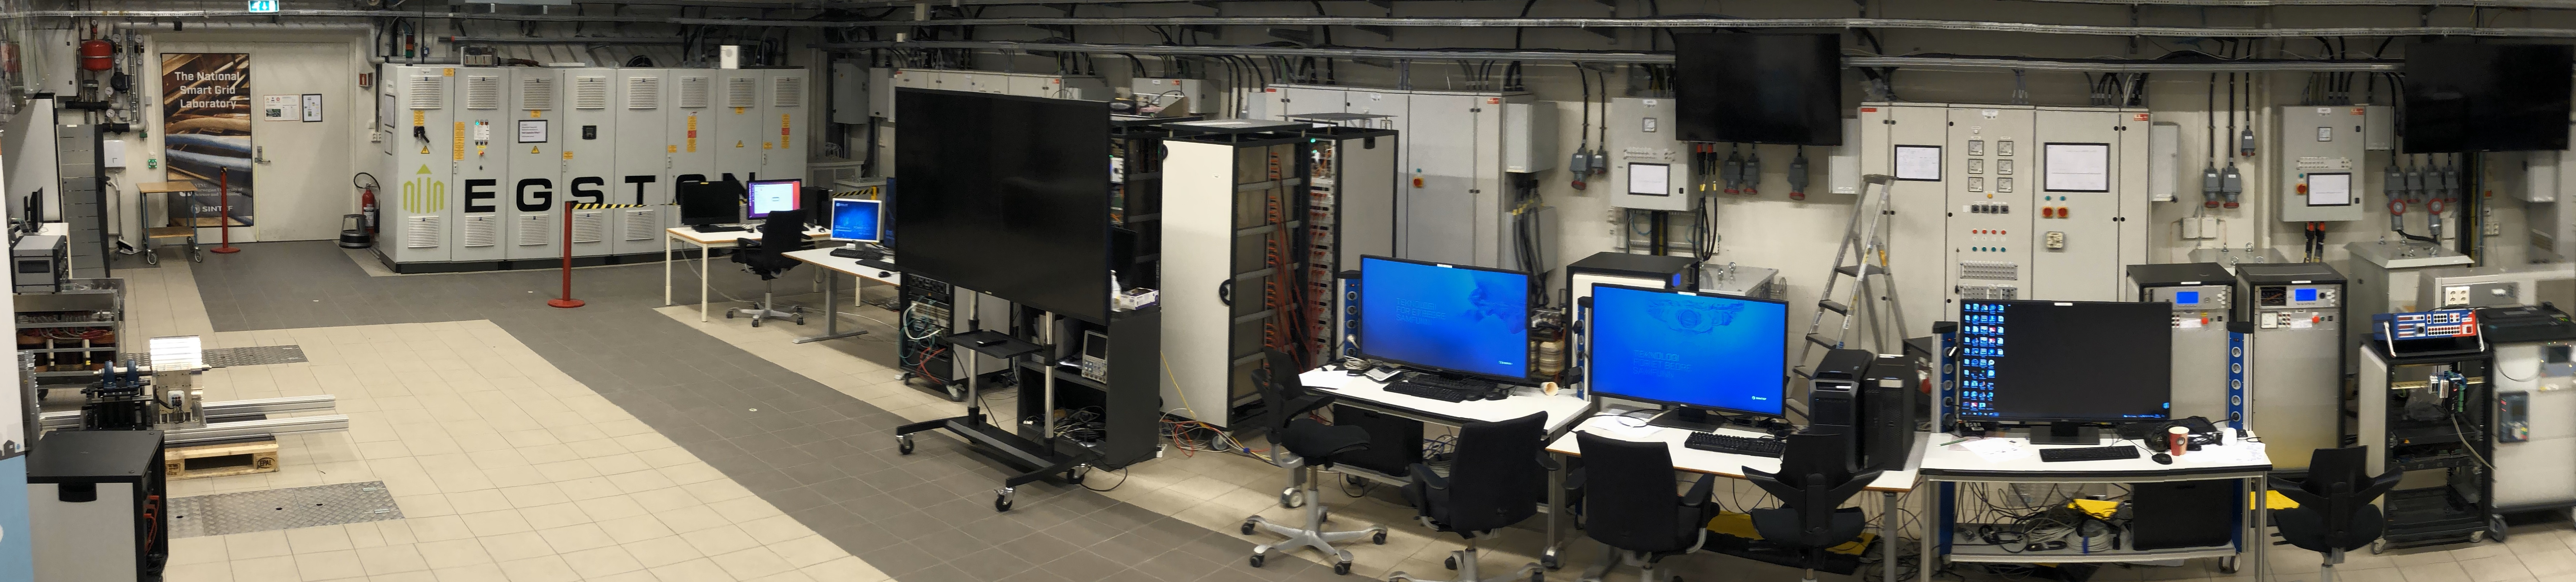
\includegraphics[width=18cm]{figures/SmartGridLab.jpg}};
	% TEXTBOXES
	\node at (-7.5,-1.5) (RTS) [caixa] {Real-Time Simulator};
	\node at (-4.5,-1.5) (GridEmu) [caixa] {Grid Emulator\\AC \& DC };
	\node at (-1.5,-1.5) (ESSTR) [caixa] {Transformer\\ESSTR};
	\node at (3.5,-1.5) (ESSGC) [caixalarga] {Power Electronic Converter\\ESSGC, ESSC$_\textrm{ac}$,
	ESSR$_\textrm{ac}$, ESSL$_\textrm{ac}$, and ESSC$_\textrm{dc}$};
	% ARROWS
	\draw [->, linha] (RTS) -- ++(0,2) -- ++(-0.75,0);
	\draw [->, linha] (GridEmu) -- ++(0,1) -- ++(-1.25,0) -- ++(0,0.65);
	\draw [->, linha] (ESSGC) -- ++(0,2.15) -- ++(2.7,0) -- ++(0,-0.5);
	\draw [->, linha] (ESSTR) -- ++(0,3) -- ++(9.25,0) -- ++(0,-1.2);
	\end{tikzpicture}

%	\ctikzset{bipoles/thickness=1}
    \ctikzset{bipoles/length=0.8cm}
    \tikzstyle{trafowind} = [circle, draw, thick, minimum size=0.4cm]
    \tikzstyle{caixa} = [rectangle, draw, thick, text width=1.6cm, text centered, minimum height=1.2cm, font=\footnotesize ]
    \tikzstyle{fonte} = [font=\footnotesize]
    \begin{tikzpicture}
    %\draw [help lines] (-1,0) grid (10,-10);
    %\node [color=gray] at (0,0) () {0,0};

    % DC grid emulator
    \node at (-2,0) (DCGridEmu) [caixa] {Grid \\ emulator \\ ac side};

    %ESS DC Link
    \draw [fonte] ($(DCGridEmu.east)+(0.7,0)$)  
        to [short, *-] ++(0,-0.4)
        to [C, l=ESSC$_\textrm{dc}$] ++(0,-0.8);
    %\fill ($(DCGridEmu.east)+(0.7,0)$) circle [radius=1pt];
    \draw [fonte] (DCGridEmu.east) to [short] (0.3,0); % , i_=$I_{dc}$
    %\node at (-0.5,0) () [anchor=south, fonte] {$V_{dc}$};

    %LSC ESS
    \foreach \x/\y in {0.7/0} 
    {
	    \node at (0.2,0.2) [shift={(\x,\y)}, rotate=0] () {$\sim$}; %{\tiny AC}; %
	    \node at (-0.2,-0.2) [shift={(\x,\y)}, rotate=0] () {$=$}; %{\tiny DC};
	    \draw [shift={(\x,\y)}, rotate=0] (-0.4,0.4) to (0.4,-0.4);
	    \draw [thick, shift={(\x,\y)}, rotate=0] (-0.4,0.4) to (0.4,0.4) to (0.4,-0.4) to (-0.4,-0.4) to (-0.4,0.4) to cycle;
    }	
    \node at (0.7,0.4) () [fonte, anchor=south] {ESSGC};

    \draw [fonte] (1.1,0) to [L, l=ESSL$_\textrm{ac}$, -*] (2.5,0); % coordinate (esscf); , i>_=$I_{ac}$
    \draw [fonte] (2.5,0) to [C, l_=ESSC$_\textrm{ac}$, *-] ++(0,-1.2); % to [R, l=$R_{ac}$]
    \draw [fonte] (3,0) to [R, l=ESSR$_\textrm{ac}$, *-] ++(0,-1.2); % to [R, l=$R_{ac}$]++(0,-0.8);
    %\node at (2.5,0) () [anchor=south, fonte] {$V_{ac}$};

    %trafo energy storage system
    \node at (3.6,0) (esstrlv) [trafowind] {};
    \node at (3.9,0) (esstrhv) [trafowind] {};
    \draw [] (2.5,0) to (esstrlv.west);

    \node at (3.75,0.15) () [anchor=south, fonte] {ESSTR};

    % DC grid emulator
    \node at (5.5,0) (ACGridEmu) [caixa] {Grid \\ emulator \\ dc side};
    \draw [] (esstrhv.east) to (ACGridEmu.west);

    \end{tikzpicture}


% CHAPTER 6 - PHIL SCALING METHOD
%\tikzstyle{caixa} = [rectangle, draw, thick,
                    text width=1.6cm, text centered, minimum height=1cm,
                    rounded corners=2, font=\footnotesize ]
\tikzstyle{legenda} = [rectangle, draw, thick,
                    text width=0.6cm, text centered, minimum height=0.35cm,
                    rounded corners=2]

\tikzstyle{fonte} = [font=\footnotesize]
\tikzstyle{cordecisao} = [fill=DaltPink] % [fill=red!15] % [fill=white] %
\tikzstyle{correinicio} = [fill=DaltGray] % [fill=blue!20]  % DaltBlue
\tikzstyle{corstart} = [fill=DaltYellow]  % [fill=yellow!20]
\begin{tikzpicture}[>=stealth]

    %%%%%%%%%%%%%%%%% X = ?? %%%%%%%%%%%%%%%%%%%%%%%%
    % Legend
    \node at (8.75,1.0) () [fonte, anchor=south] {\textbf{Gate types}};
    \node at (9.0,0.8) (legstart) [legenda, corstart] {};
    \node at (legstart.east) [fonte, anchor=west] {Start};
    
    \node at (9.0,0.2) (legrestart) [legenda, correinicio] {};
    \node at (legrestart.east) [fonte, anchor=west] {Selection};

    \node at (9.0,-0.4) (legcalc) [legenda] {};
    \node at (legcalc.east) [fonte, anchor=west] {Calculations};

    \node at (9.0,-1.0) (legeval) [legenda, cordecisao] {};
    \node at (legeval.east) [fonte, anchor=west] {Decisions};

    \draw [->, densely dotted, thick] (legeval.west) to ++(-0.35,0) to ++(0,1.2) to ++(0.35,0);
    \draw [->, densely dotted, thick] (legstart) to (legrestart);
    \draw [->, densely dotted, thick] (legrestart) to (legcalc);
    \draw [->, densely dotted, thick] (legcalc) to (legeval);
    
    \draw [] (7.75,1.5) to (11.25,1.5) to (11.25,-1.4) to (7.75,-1.4) to cycle;

    %\draw [] (-4.5,2.75) to (19,2.75) to (19,-6.75) to (-4.5,-6.75) to cycle;
    %\draw [] (-2.9,2.75) to (17.25,2.75) to (17.25,-6.75) to (-2.9,-6.75) to cycle;
        
    %%%%%%%%%%%%%%%%% X = 0 %%%%%%%%%%%%%%%%%%%%%%%%
    % DC voltage
    \node at (0,0) (Vdc) [caixa, cordecisao] {Evaluate \\ $V_{bdc}^{sd}$};
    % \node at (Vdc.north) () [fonte, anchor=south west] {dc path $\downarrow$};
    \node at (Vdc.north west) [fonte, anchor=south west] () {$V_{bdc}^{sd} = V_{bac}^{sd} \: \dfrac{V_{bdc}^{f\!s}}{V_{bac}^{f\!s}}$};

    % DC current
    \node at (0,-2) (Idc) [caixa, cordecisao] {Evaluate \\ $I_{bdc}^{sd}$};
    \node at (Idc.south) [fonte, anchor=north] () {$ I_{bdc}^{sd} = \dfrac{S_{b}^{sd}}{V_{bdc}^{sd}}$}; 

    % Cdc
    \node at (0,-4) (Cdc) [caixa, cordecisao] {Choose \\ $C_{dc}^{sd}$};
    \node at (Cdc.south west) () [fonte, anchor=north west] {$\dfrac{C_{dc}^{sd}{{V_{bdc}^{sd}}^2}}{2 S_{b}^{sd}}
    \approx
    \dfrac{C_{dc}^{f\!s}{{V_{bdc}^{f\!s}}^2}}{2 S_{b}^{f\!s}}$}; % H^{sd}

    %%%%%%%%%%%%%%%%% X = 4 %%%%%%%%%%%%%%%%%%%%%%%%
    \node at (4,2) (inicio) [caixa, corstart] {Full-Scale \\ Parameters};
    %\node at (inicio.west) () [fonte, anchor=east] {$S_{b}^{f\!s}, V_{bac}^{f\!s}, I_{bac}^{f\!s}, Z_{b}^{f\!s}, L_{b}^{f\!s}, C_{b}^{f\!s}$};
    \node at (inicio.east) () [fonte, anchor=west] {$S_{b}^{f\!s}, V_{bac}^{f\!s}, I_{bac}^{f\!s}, Z_{b}^{f\!s}, L_{b}^{f\!s}, C_{b}^{f\!s}, V_{bdc}^{f\!s}, I_{bdc}^{f\!s}, C_{dc}^{f\!s}, H^{f\!s}$};
    
    % Ensure 
    %\node at (4,0) (acdc) [caixa] {Calculate \\ $V_{bdc}^{sd}$};
    %\node at (acdc.north) [fonte, anchor=south] () {$\dfrac{V_{bdc}^{sd}}{V_{bac}^{sd}} = \dfrac{V_{bdc}^{f\!s}}{V_{bac}^{f\!s}}$};
    
    % AC voltage
    \node at (4,0) (Vac) [caixa, correinicio] {Select \\ $V_{bac}^{sd}$, $I_{bac}^{sd}$};    
    % \node at (Vac.north) () [fonte, anchor=south east] {ac path $\downarrow$};

    
    % Sn
    \node at (4,-2) (Sn) [caixa] {Calculate \\ $S_{b}^{sd}$};
    \node at (Sn.east) [fonte, anchor=west] () {$ S_{b}^{sd} = \sqrt{3} V_{bac}^{sd} I_{bac}^{sd}$};
    
    % pu bases
    % \node at (4,-4) (puBases) [caixa] {Calculate \\ $Z_{b}^{sd}\!,L_{b}^{sd}\!,C_{b}^{sd}$};

    % pu bases   %Z_{b}=\dfrac{V_{bac}}{\sqrt{3} I_{bac}}, L_{b}=\dfrac{V_{bac}}{\omega_{n} \sqrt{3} I_{bac}}, C_{b} = \dfrac{\sqrt{3} I_{bac}}{\omega_n V_{bac}}   % 
    % \node at (puBases.north) [fonte, anchor=south, text width=2.5cm, text centered ] () { $Z_{b}=\dfrac{V_{bac}}{\sqrt{3} I_{bac}} $ \\ $L_{b}=\dfrac{V_{bac}}{\omega_{n} \sqrt{3} I_{bac}}$ \\ $C_{b}= \dfrac{\sqrt{3} I_{bac}}{\omega_n V_{bac}}$};
     \node at (4,-4) (puBases) [caixa] {Calculate \\ $Z_{b}^{sd}\!,L_{b}^{sd}\!,C_{b}^{sd}$};

    % Cac
    \node at (4,-8) (Cac) [caixa, cordecisao] {Choose \\ $C_{ac}^{sd}$};
    \node at (Cac.west) () [fonte, anchor=east] {$\dfrac{C_{ac}^{sd}}{ C_{b}^{sd}} \approx \dfrac{C_{ac}^{f\!s}}{ C_{b}^{f\!s}}$};
    
    %%%%%%%%%%%%%%%%% X = 7.5 %%%%%%%%%%%%%%%%%%%%%%%%
    % Converter reactor
    \node at (7.5,-4) (L1) [caixa, cordecisao] {Choose \\ $L_{r}^{sd}$};
    \node at (L1.north) () [fonte, anchor=south] {$\dfrac{L_{r}^{sd}}{ L_{b}^{sd}} \approx \dfrac{L_{r}^{f\!s}}{ L_{b}^{f\!s}}$}; % \eqref{eq:Compare_lr}

     % Transformer Lac, Ltr
    \node at (7.5,-6) (Ltr) [caixa, cordecisao] {Choose \\ $L_{t}^{sd}$};
    \node at (Ltr.north west) () [fonte, anchor=south] {$\dfrac{L_{t}^{sd}}{ L_{b}^{sd}} \approx \dfrac{L_{t}^{f\!s}}{ L_{b}^{f\!s}}$};

    % fres
    \node at (7.5,-8) (fres) [caixa, cordecisao] {Evaluate \\ $F_{\textrm{res}}^{sd}$};
    \node at (fres.north west) () [fonte, anchor=south] {$F_{\textrm{res}}^{sd} \approx F_{\textrm{res}}^{f\!s}$};
    
    %%%%%%%%%%%%%%%%% X = 11 %%%%%%%%%%%%%%%%%%%%%%%%
    % Converter reactor
    \node at (10.5,-4) (Rac) [caixa, cordecisao] {Evaluate \\ $R_{r}^{sd}$};
    \node at (Rac.north) () [fonte, anchor=south] {$\dfrac{R_{r}^{sd}}{ Z_{b}^{sd}} \approx \dfrac{R_{r}^{f\!s}}{ Z_{b}^{f\!s}}$}; %  \eqref{eq:rrsdpu}
    
    \node at (10.5,-6) (Rtr) [caixa, cordecisao] {Evaluate \\ $R_{t}^{sd}$};
    \node at (Rtr.north) () [fonte, anchor=south] {$\dfrac{R_{t}^{sd}}{ Z_{b}^{sd}} \approx \dfrac{R_{t}^{f\!s}}{ Z_{b}^{f\!s}}$};
    
    %% Rshunt
    %\node at (-4,-8) (Rshunt) [caixa] {Choose \\ $R_{bac}^{sd}$};
    %\node at (Rshunt.north) () [fonte, anchor=south] {$\dfrac{R_{bac}^{sd}}{ Z_{b}^{sd}} \approx \dfrac{R_{bac}^{f\!s}}{ Z_{b}^{f\!s}}$ \eqref{eq:Rac}};
    
    %%%%%%%%%%%%%%%% AC CONNECTORS %%%%%%%%%%%%%%%%%%%%%%%%
    % AC connectors, and crossovers to DC
    \draw [fonte, ->] (inicio) to (Vac);
    
    %\draw [fonte, ->] (Vac) to (acdc);
    
    \draw [fonte, ->] (Vac) to
        node [fonte, pos=0.0, anchor=south east] () {DC voltage $\leftarrow$}
        (Vdc);
  
    \draw [fonte, ->] (Vac) to node [fonte, pos=0.0, anchor=north west] () {$\downarrow$ AC power} (Sn);
    
    \draw [fonte, ->] (Sn) to node [fonte, pos=0.0, anchor=north west] () {$\downarrow$ LCL filter} (puBases);
    \draw [fonte, ->] (Sn) to node [fonte, pos=0.0, anchor=south east] () {DC side $\leftarrow$} (Idc);
    \draw [fonte, ->] ($(Sn) + (-2.2,0)$) |- ($(Cdc.east)+(0,-0.15)$);
    \filldraw [black] ($(Sn) + (-2.2,0)$) circle (1pt);
    
    \draw [fonte, ->] (puBases) to node [fonte, pos=0.0, anchor=south west ] () {$\rightarrow$ Reactor} (L1);
    \draw [fonte, ->] (puBases) to (Cac);
    \draw [fonte, ->] ($(puBases) + (0,-2)$) to 
        node [fonte, pos=0, anchor=south west] () {$\rightarrow$ Transformer}
        node [fonte, pos=0, anchor=north east] () {Shunt branch $\downarrow$ } (Ltr);
    \filldraw [black] ($(puBases) + (0,-2)$) circle (1pt);
    
    \draw [fonte, ->] (L1) to (Rac);
    \draw [fonte, ->] ($(L1.south)+(0.5,0)$) to ($(L1)+(0.5,-1)$) to ++(1.3,0) |- ($(fres.east)+(0,0)$);
    
    \draw [fonte, ->] (Ltr) to (Rtr);
    \draw [fonte, ->] ($(Ltr.south)+(0.5,0)$) to ($(Ltr)+(0.5,-1)$) to ++(1,0) |- ($(fres.east)+(0,0.3)$);

    %\draw [fonte, ->] ($(Cac.east)+(0,-0.3)$) to ($(fres.west)+(0,-0.3)$);
    \draw [fonte, ->] (Cac.east) to (fres.west);

    %\draw [fonte, ->] (fres) to (Rshunt);

    %%%%%%%%%%%%%%%% DC CONNECTORS %%%%%%%%%%%%%%%%%%%%%%%%
    % DC connectors
    % \draw [fonte, ->] (inicio.east) -| (Vdc.north);
    \draw [fonte, ->] (Vdc) to node [fonte, pos=0, anchor=north west] () {$\downarrow$ DC current} (Idc);
    \draw [fonte, ->] ($(Vdc) + (0,-1)$) to ++(1.5,0) |- ($(Cdc.east)+(0,0.15)$);
    \filldraw [black] ($(Vdc) + (0,-1)$) circle (1pt);

\end{tikzpicture}
%\ctikzset{bipoles/thickness=1}
\ctikzset{bipoles/length=0.8cm}
\tikzstyle{trafowind} = [circle, draw, thick, minimum size=0.4cm]
\tikzstyle{caixa} = [rectangle, draw, thick, text width=1.6cm, text centered, minimum height=1.2cm, font=\footnotesize ]
\tikzstyle{fonte} = [font=\footnotesize]
\begin{tikzpicture}
    %\draw [help lines] (-1,0) grid (10,-10);
    %\node [color=gray] at (0,0) () {0,0};

    % DC grid emulator
    \node at (-2,0) (DCEmuPic) {
\includegraphics[width=0.5cm]{figures/battery.pdf}};

    \node at (-2,0) (DCGridEmu) [caixa] {}; %dc \\ grid \\ emulator
    \node at (DCGridEmu.north) [fonte, anchor=south] () {Battery model}; % ac \\ grid \\ emulator
    \node at (DCGridEmu.south) [fonte, anchor=north] () {DC grid emulator}; % ac \\ grid \\ emulator

    %ESS DC Link
    \draw [fonte] (DCGridEmu.east) to [short] (-0.5,0) to [C, l=$C_{dc}$] ++(0,-1.2);
    \draw [fonte] (-0.5,0) to [short, i_=$I_{dc}$] (0.3,0);
    \node at (-0.5,0) () [anchor=south, fonte] {$V_{dc}$};
    \fill (-0.5,0) circle [radius=1pt];

    %LSC ESS
    \foreach \x/\y in {0.7/0}
    {
	    \node at (0.2,0.2) [shift={(\x,\y)}, rotate=0] () {$\sim$}; %{\tiny AC}; %
	    \node at (-0.2,-0.2) [shift={(\x,\y)}, rotate=0] () {$=$}; %{\tiny DC};
	    %\node at (0.4,0.15) () [anchor=west, fonte, shift={(\x,\y)}, rotate=0] {ESSGC};
	    %\node at (0.4,-0.15) () [anchor=west, fonte, shift={(\x,\y)}, rotate=0] {\SI{10}{\mega \voltampere}};
	    %\node at (0.4,0) () [anchor=west, fonte, shift={(\x,\y)}, rotate=0] {ac/dc};
	    \draw [shift={(\x,\y)}, rotate=0] (-0.4,0.4) to (0.4,-0.4);
	    \draw [thick, shift={(\x,\y)}, rotate=0] (-0.4,0.4) to (0.4,0.4) to (0.4,-0.4) to (-0.4,-0.4) to (-0.4,0.4) to cycle;
	    \node at (0,0.4) [fonte,anchor=south,shift={(\x,\y)}, rotate=0] () {PEC};
    }	

    \draw [fonte] (1.1,0) to [L, l=${L_{r},R_r}$, i>_=$I_{ac}$] (2.5,0); % coordinate (esscf); 
    \draw [fonte] (2.5,0) to [short, i>_=${P,Q}$] (2.6,0); % coordinate (esscf); 
    \draw [fonte] (3,0) to [C, l=$C_{ac}$] ++(0,-1.2);
    \node at (3,0) () [anchor=south, fonte] {$V_{ac}$};
    \fill (3,0) circle [radius=1pt];

    %trafo energy storage system
    \node at (3.55,0) (esstrlv) [trafowind] {};
    \node at (3.85,0) (esstrhv) [trafowind] {};
    \draw [] (2.6,0) to (esstrlv.west);

    \node at (3.7,0.15) () [anchor=south, fonte] {$L_{t} \: R_{t}$};

    % DC grid emulator
    \node at (5.25,0) (ACEmuPic) {
\includegraphics[width=1.1cm]{figures/smartgrid.pdf}};
    \node at (5.25,0) (ACGridEmu) [caixa] {}; % ac \\ grid \\ emulator
    \node at (ACGridEmu.north) [fonte, anchor=south] () {Grid model}; % ac \\ grid \\ emulator
    \node at (ACGridEmu.south) [fonte, anchor=north] () {AC grid emulator}; % ac \\ grid \\ emulator
    \draw [] (esstrhv.east) to (ACGridEmu.west);

\end{tikzpicture}
%\tikzstyle{linha} = [line width=1.05mm, rounded corners=1mm, yellow!60]
\tikzstyle{caixa} = [rectangle, draw=yellow!60, fill=yellow!60, text width=2cm, text centered, minimum height=0.75cm, font=\footnotesize, rounded corners] 
\tikzstyle{caixalarga} = [rectangle, draw=yellow!35, fill=yellow!60, text width=6cm, text centered, minimum height=0.75cm, font=\footnotesize, rounded corners ]
\begin{tikzpicture}[>={Triangle[angle=60:3mm]}]
 % PICTURE
    \node at (0,0) (LabPick) {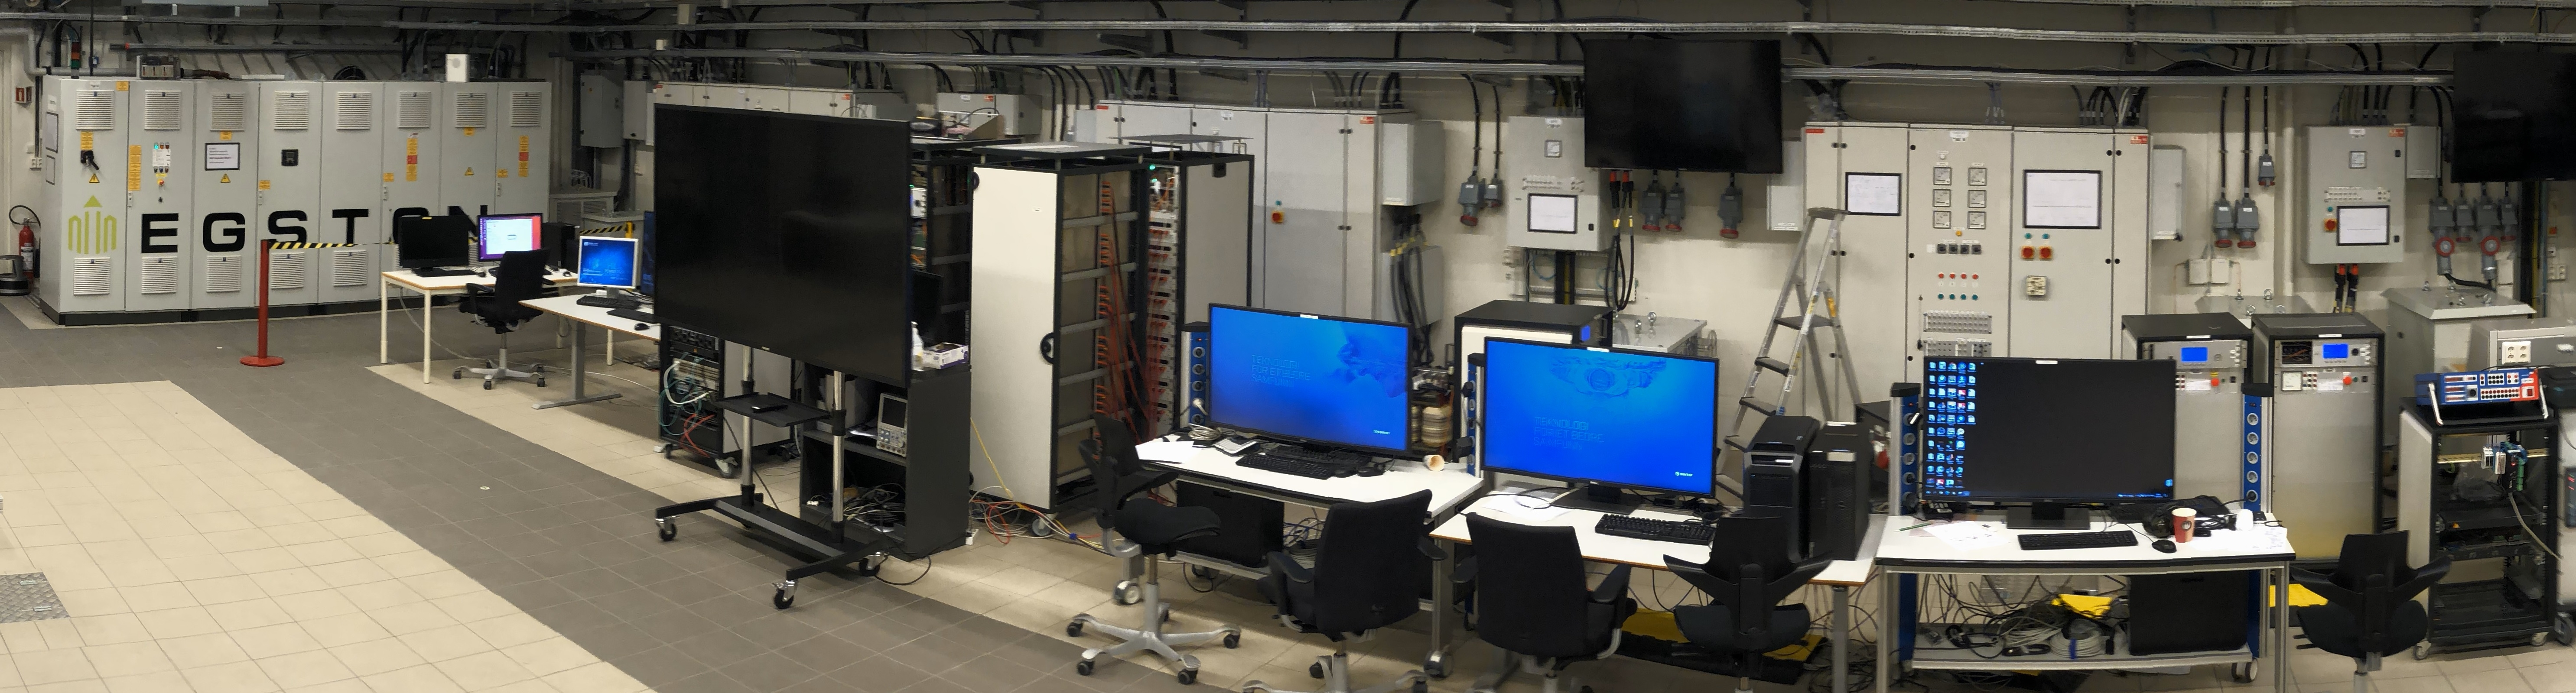
\includegraphics[width=18cm]{figures/SmartGridLabNarrower.jpg}};
	% TEXTBOXES
	\node at (-7.5,-0.8) (GridEmu) [caixa] {Grid Emulator\\ac \& dc };
	\node at (-1.5,1.5) (ESSTR) [caixa] {Transformer\\$L_t$ and $R_t$};
	%\node at (3.5,-1.8) (ESSGC) [caixalarga] {Power Electronic Converter (PEC)\\ plus $C_{dc}$, $L_r$, $R_r$, and $C_{ac}$};
    \node at (3.5,1.5) (ESSGC) [caixalarga] {Power Electronic Converter (PEC)\\ plus $C_{dc}$, $L_r$, $R_r$, and $C_{ac}$};
	
 % ARROWS
	\draw [->, linha] (GridEmu) -- ++(0,1);
	\draw [->, linha] (ESSGC) -- ++(0,-0.8) -- ++(2.7,0) -- ++(0,-0.4);
	\draw [->, linha] (ESSTR) -- ++(0,0.7) -- ++(9.6,0) -- ++(0,-1.8);
	
	%\node at (10.9,0) (ConvScopePick) {\includegraphics[width=3.6339165cm]{figures/ConverterAndScope.jpg}};
    %\node at (0,-5) (ConvScopePick) {\includegraphics[width=3.6339165cm]{figures/ConverterAndScope.jpg}};
    \node at (0,-5.2) (ConvScopePick) {\includegraphics[width=4cm]{figures/ConverterAndScope.jpg}};
	
	\draw [line width=0.25mm, yellow!90] (5.8,0.25) --
	    ++(1,0) --
	    ++(0,-0.7) --
	    ++(-1,0) -- cycle;
	
    %\draw [line width=0.25mm, yellow!90] ($(5.8,0.25)+(1,0)$) -- (9.1, 2.42261104);
	%\draw [line width=0.25mm, yellow!90] ($(5.8,0.25)+(1,-0.7)$) -- (9.1, -2.42261104);

    \draw [line width=0.25mm, yellow!90] ($(5.8,0.25)+(0,0)$) -- (-2, -2.52);
    \draw [line width=0.25mm, yellow!90] ($(5.8,0.25)+(1,-0.7)$) -- (2, -7.87);
 
	\node at (0,-5.5) (ConvScope) [caixa] {PEC with\\ Oscilloscope};
	
\end{tikzpicture}


\end{document}